%%%% ijcai11.tex
% For ICDM: Jaiwei Han's formula?
% Ideas for intro: what is new? Motivate each component. 
% for background: move other models to semantics section.
% mention MLN-Boost.
% conditional probabilities are motivated by Heckerman et al.
% future work: worry about consistency
% combining rules also have scale problem, same as with aggregation.
% MLN-boost: scalability problems
% baseline model: researchers, users. Move boosting to related work. Not two different examples. 
% Blind review? Are references free?
% semantics and the relationship to the standard BN equation.
% structure learning is fast with LAJ.
% Local probability models, use terminology from Heckermann.

\typeout{IJCAI-13 Instructions for Authors}

% These are the instructions for authors for IJCAI-13.
% They are the same as the ones for IJCAI-11 with superficical wording
%   changes only.

\documentclass{article}
% The file ijcai13.sty is the style file for IJCAI-13 (same as ijcai07.sty).
\usepackage{ijcai13}
\usepackage{graphicx} 
\usepackage{ltexpprt}
% Use the postscript times font!
\usepackage{times}

%Example for automatically rescaling equations. 
% This is very tricky.
%\begin{equation}
%\label{eq:pimax}
%\resizebox{.55\textwidth}{!}{$
%\begin{split}
%P(\jtable_{2}|\set{E},\ttable) \propto &
%P(\keys = [jack,101],\it{Gr} = A, \it{Sat} = 1|\it{Int} = \class, \it{Rank} = 1, \it{Rat} = 3, \it{Diff}=1)\\
%\times & P(\keys = [jack,102],\it{Gr} = B, \it{Sat} = 2|\it{Int} = \class, \it{Rank} = 1, \it{Rat} = 2, \it{Diff}=2).
%\end{split}$
%}
%\end{equation}

%\usepackage{times}
%\usepackage[normaltitle,normalbib,normalmargins,normalindent]{savetrees}
\usepackage{amsmath}
\usepackage{amsfonts}
\usepackage{amssymb}
\usepackage{graphicx}
\usepackage{url}
%\usepackage{subfigure}
\usepackage{epstopdf}
\setcounter{MaxMatrixCols}{30}
%\usepackage{algorithm}
%\usepackage{algorithmic}
\usepackage{subfigure}
%\usepackage{subcaption}
\usepackage{fancyhdr}
\graphicspath{{../}{figures/}}
\usepackage{todonotes}

\DeclareMathOperator*{\argmax}{argmax}
\DeclareMathOperator*{\argmin}{argmin}
%\DeclareMathOperator{\pattern}{\pi}
\DeclareMathOperator{\Poly}{\mathbf{\mathrm{P}}}
\DeclareMathOperator{\RP}{\mathbf{\mathrm{RP}}}
%\DeclareMathOperator{\FP}{\mathbf{\mathrm{FP}}}
\DeclareMathOperator{\NP}{\mathbf{\mathrm{NP}}}
%\DeclareMathOperator{\E}{\mathbb{E}}
\renewcommand{\d}{\mathbf{d}}

\newcommand{\ZZ}{\mathbf{Z}}

\newcommand{\indep}{\ensuremath{\perp{}\!\!\!\!\!\!\!\perp{}}}
\newcommand{\dep}{\ensuremath{{\perp{}\!\!\!\!\!\!\!\not  \perp{}}}}
%\renewcommand{\L}{\mathcal{L}}
% variables denoting sets of nodes
\newcommand{\V}{V} 
\newcommand{\partC}{\mathcal{C}}
\newcommand{\pattern}{\pi}
% variables denoting nodes
\newcommand{\B}{B}
\renewcommand{\P}{P}
\newcommand{\R}{R}
\newcommand{\X}{X}
\newcommand{\Y}{Y}
\newcommand{\Z}{Z}
\newcommand{\F}{F}
\newcommand{\U}{U}
\newcommand{\W}{W}
\renewcommand{\S}{S}
\newcommand{\C}{C}
\newtheorem{mydef}{Proposition}
%variables for values
%\newcommand{\u}{u}
\renewcommand{\a}{a}
\renewcommand{\b}{b}
\newcommand{\z}{z}
\renewcommand{\v}{v}
\newcommand{\x}{x}
\newcommand{\y}{y}
\newcommand{\p}{p}
\newcommand{\s}{s}
\newcommand{\w}{w} % weights


%statistics
\newcommand{\divergence}{\it{D}}
\newcommand{\score}{\it{score}}
\newcommand{\confidence}{\it{conf}}
\newcommand{\support}{\it{support}}
\newcommand{\loglikelihood}{\it{LOG}}
\newcommand{\lof}{\it{LOF}}
\newcommand{\llmetric}{-L}
\newcommand{\lr}{\it{LR}}
\newcommand{\kl}{\it{KL}}
\newcommand{\el}{\it{EL}}
\newcommand{\mi}{\it{MI}}
\renewcommand{\mid}{\it{ELD}}
\newcommand{\jid}{\it{JID}}
\newcommand{\roc}{\it{ROC}}
\newcommand{\outrank}{\it{OutRank}}
\newcommand{\knn}{\it{KNNOutlier}}
\newcommand{\auc}{\it{AUC}}
\newcommand{\eld}{\it{ELD}}
\newcommand{\fd}{\it{FD}}
\newcommand{\parameter}{\theta}
\newcommand{\parameters}{\bs{\parameter}}
\newcommand{\bic}{\mathit{BIC}}
%random variables and graphical models
% number of values in the domain of a random variable
% variables for BNs
\newcommand{\domvals}{k}
\newcommand{\nodevalue}{\v}
\newcommand{\parvalue}{\mathbf{\pi}} % a single assignment of values to a set of 
%parents
\newcommand{\parvals}{l} % number of values of parent state.
\renewcommand{\r}{r} % CP-table row
\newcommand{\nbhd}{{\mathsf {nbdh}}}
\newcommand{\child}{\mathit{child}}
\newcommand{\parent}{\mathit{pa}}
\newcommand{\parents}{\mathbf{pa}}
\newcommand{\Parents}{\mathbf{PA}}
\newcommand{\family}{F} % families, family formulas
\newcommand{\vpi}{\mathbf{pa}} % for vectors of variable assignments
\renewcommand{\l}{\ell} % class label
\newcommand{\states}{r} % number of states of a variable
%\newcommand{\value}{value}
\newcommand{\mb}{\set{mb}} % markov blanket of a variable, vector-valued
\newcommand{\ssize}{N} % number of rows in join table; size of sample
\newcommand{\mbstates}{m} % number of states in Markov blanket
\newcommand{\frequency}{fr}
\newcommand{\pseudo}{\ast}
\newcommand{\counts}{+}
\newcommand{\weighted}{\ast}
\newcommand{\halpern}{H}
\newcommand{\Thetaa}{\theta}
\newcommand{\instance}{I}

%logic notation
%\newcommand{\predicate}{\phi}
\newcommand{\functor}{f}
\newcommand{\outdomain}{V}
\newcommand{\indomain}{\Omega}
\newcommand{\variable}{X} % first-order variable
\newcommand{\population}{\mathcal{P}}
\newcommand{\entity}{x}
\newcommand{\formula}{\phi}
\newcommand{\formulas}{\mathcal{\phi}}
\newcommand{\literal}{l}
\newcommand{\conjunction}{\set{C}} % conjunction of literals
\newcommand{\fterm}{\f} % open function term
\newcommand{\fterms}{F} % set of function terms, also nodes in JBN
\newcommand{\term}{\sigma}
\newcommand{\Terms}{\bs{\sigma}}
\newcommand{\constant}{a}
\newcommand{\constants}{\bs{\constant}}
\newcommand{\gterm}{g} % ground term
\newcommand{\gterms}{\bs{\gterm}} %list of ground terms
\newcommand{\vterm}{x} % variable term
\newcommand{\vterms}{\bs{\vterm}} % list of variable terms
\newcommand{\assign}{A} % assignment of values to Bayes net
\newcommand{\resultset}{\mathbb{R}}
\newcommand{\grounds}{\#}
\newcommand{\grounding}{\gamma}
\newcommand{\groundall}{\Gamma}
\newcommand{\vars}{\mathit{Var}} % variables in a conjunction
\newcommand{\igraph}{I} % instance-level dependency graph.
\newcommand{\assignment}{\set{a}}
\newcommand{\atom}{\ell}
\newcommand{\gnode}{\alpha}
\newcommand{\gfamily}{\ground{f}}
\newcommand{\numformulas}{m}
\newcommand{\structure}{\mathcal{S}}
% logic programs
\newcommand{\program}{\mathcal{B}}
\newcommand{\clause}{\mathcal{c}}
\newcommand{\head}{\mathit{head}}
\newcommand{\body}{\mathit{body}}
\newcommand{\crule}{\mathit{cr}} % combining rule
\newcommand{\level}{\mathit{level}} % rank of function symbols in LP

%datbase schema
\newcommand{\rcolumns}{R}
\newcommand{\ecolumns}{E}
\newcommand{\dtable}{T} % can't use \table. Generic database table
\newcommand{\datatable}{D} % generic data table, not necessarily part of database.
\newcommand{\jtable}{J} % join table
\newcommand{\Ejoin}{$J^{+}$}
\newcommand{\jtables}{m}
\newcommand{\rtable}{R} % relationship table
\newcommand{\etable}{E} % entity table.
\newcommand{\ttable}{X} % target table
\newcommand{\nextended}{n}
\newcommand{\row}{r}
\newcommand{\rows}{\mathit{rows}}
\newcommand{\col}{j}
\newcommand{\cols}{\mathit{cols}}
\newcommand{\unary}{\f} % to denote a unary or attribute function
\newcommand{\numatts}{u} % to denote the number of unary or attribute functions.
\newcommand{\g}{g} % alternative for function
\newcommand{\relational}{\mathbf{r}} % denotes a generic relational functors, can be both relationship or descriptive attribute of relationship
\newcommand{\Relation}{R} % denotes a generic boolean relation
% a special type of literal conjunction that assigns a value %to each variable
\providecommand{\keywords}{\textbf{keywords: }}
\newcommand{\loss}{\ell}
\newcommand{\class}{c} % the class attribute
\newcommand{\classlabel}{y} % the class label
\newcommand{\classifier}{\mathcal{M}}
\newcommand{\target}{t} % target object
\newcommand{\Target}{T}
\newcommand*\rfrac[2]{{}^{#1}\!/_{#2}}
\newcommand{\object}{o}
\newcommand{\Class}{C}
\newcommand{\scorediff}{\Delta}
\newcommand{\model}{B}
\newcommand{\modelprob}{\theta}
\newcommand{\profile}{P}
% the probabilities defined by a model, like conditional probabilities in a BN
\newcommand{\Targetcount}{\Gamma}
\newcommand{\neighbor}{n}
\newcommand{\feature}{V} % feature or desc attribute of object or link
\newcommand{\features}{\bs{v}} % features 
\newcommand{\Features}{\bs{V}}
\newcommand{\attribute}{a} % nonclass attribute of target object
\newcommand{\attributes}{\bs{a}}
\newcommand{\rels}{\bs{R}} % chain of relationships.
\newcommand{\maxpath}{\rho}
\newcommand{\eatts}{\it{1Nodes}}
\newcommand{\ratts}{\it{2Nodes}}
\newcommand{\atts}{\it{ANodes}}
\newcommand{\marginalize}{\it{margin}}
%special functions
\newcommand{\AVG}{\it{AVG}}
\newcommand{\instances}{n} % counts number of occurrences in DB
\newcommand{\prob}{p} % frequency of formula true in in DB

%variables denoting graphs or models
\newcommand{\mln}{M}
\newcommand{\G}{G}
\newcommand{\node}{V}
\newcommand{\nodes}{V}
\newcommand{\edges}{E}
\newcommand{\clique}{C}
\newcommand{\cliques}{\mathcal{\clique}}
\newcommand{\cliquevalue}{c}
\newcommand{\graph}{G}
\newcommand{\M}{M}
\newcommand{\J}{J}
\renewcommand{\H}{H}
\newcommand{\K}{K} % component
\renewcommand{\O}{O} % oracle
\renewcommand{\path}{\rho} % path, also foreignkey path
% Markov nets
\newcommand{\potential}{\Psi}
% database schema
\newcommand{\type}{\tau} % to denote a generic type
\newcommand{\E}{E} % for entity tables
\newcommand{\e}{e} % for specific entities
\newcommand{\f}{f}
\newcommand{\new}{\it{new}}
\renewcommand{\c}{c}
\renewcommand{\R}{R} % for relationship tables
\newcommand{\A}{A} % for attributes
\newcommand{\T}{T} % for tables generically
\newcommand{\New}{N}
\newcommand{\D}{\mathcal{D}} % for database instance
\newcommand{\databases}{\set{D}} % the number of databases
\newcommand{\vocab}{\mathcal{\L}} % for logical vocabulary associated with database
\newcommand{\name}{\mathit{name}} % generic attribute
\newcommand{\dom}{\mathit{dom}} % domain of attributes
\newcommand{\etables}{\alpha} % entity tables
\newcommand{\rtables}{\beta} % relationship table number
% specific constructs for examples


\newcommand{\team}{\it{T}}
\newcommand{\player}{\it{P}}
\newcommand{\match}{\it{M}}


\newcommand{\director}{\it{Director}}
\newcommand{\movie}{\it{Movie}}
\newcommand{\user}{\it{User}}
\newcommand{\corr}{\it{\rho}}
\newcommand{\student}{\mathit{Student}}
\newcommand{\I}{\mathit{I}}
\newcommand{\course}{\mathit{Course}}
\newcommand{\prof}{\mathit{Professor}}
\newcommand{\person}{\mathit{Person}}
\newcommand{\TA}{\mathit{TA}}
\newcommand{\actor}{\mathit{Actor}}
\newcommand{\age}{\mathit{age}}
\newcommand{\intelligence}{\mathit{intelligence}}
\newcommand{\diff}{\mathit{difficulty}}
\newcommand{\reg}{\mathit{Registered}}
\newcommand{\win}{\it{win}}
\newcommand{\ra}{\mathit{RA}}
\newcommand{\bt}{\mathit{blood type}}
\newcommand{\grade}{\mathit{grade}}
\newcommand{\gpa}{\mathit{gpa}}
\newcommand{\jack}{\mathit{Jack}}
\newcommand{\jill}{\mathit{Jill}}
\newcommand{\smith}{\mathit{Smith}}
\newcommand{\cmpt}{\mathit{CMPT120}}
\newcommand{\hi}{\mathit{Hi}}
% various constants
\newcommand{\true}{\mathit{T}}
\newcommand{\false}{\mathit{F}}
\newcommand{\normalconstant}{Z} % the normalization constant

% orderings
\newcommand{\pred}{\mathit{pred}}
%procedure names and such
\newcommand{\join}{\textsc{Join-Frequencies}}
\newcommand{\linus}{\textsc{Linus }}
\newcommand{\foil}{\textsc{Foil }}
\newcommand{\MLN}{\textsc{MLN}}
\newcommand{\treetilde}{\textsc{TILDE }}

%%%
%undirected models
\newcommand{\pot}{\phi} % potential function
%\newcommand{\theHalgorithm}{\arabic{algorithm}}
\newcommand{\test}{test}
\def\set#1{\mathbf{#1}}
\def\bs#1{\boldsymbol{#1}}
\def\ground#1{\overline{#1}}


\newcommand{\MLNA}{\textsc{MSL}}
\newcommand{\MLNConst}{\textsc{MSLc}}
\newcommand{\LHL}{\textsc{LHL}}
\newcommand{\LHLConst}{\textsc{LHLc}}
% the following package is optional:
%\usepackage{latexsym} 

% Following comment is from ijcai97-submit.tex:
% The preparation of these files was supported by Schlumberger Palo Alto
% Research, AT\&T Bell Laboratories, and Morgan Kaufmann Publishers.
% Shirley Jowell, of Morgan Kaufmann Publishers, and Peter F.
% Patel-Schneider, of AT\&T Bell Laboratories collaborated on their
% preparation.

% These instructions can be modified and used in other conferences as long
% as credit to the authors and supporting agencies is retained, this notice
% is not changed, and further modification or reuse is not restricted.
% Neither Shirley Jowell nor Peter F. Patel-Schneider can be listed as
% contacts for providing assistance without their prior permission.

% To use for other conferences, change references to files and the
% conference appropriate and use other authors, contacts, publishers, and
% organizations.
% Also change the deadline and address for returning papers and the length and
% page charge instructions.
% Put where the files are available in the appropriate places.
% add plates to emphasize groundings.
% check Poole on learning ordering for Gibbs sampling.

\title{A Log-Linear Model for Bayes Nets Applied to Relational Data}
%\author{Oliver Schulte , Hassan Khosravi , Yuke Zhu \and Tianxiang Gao \\
%School of Computing Science,Simon Fraser University\\
%Vancouver-Burnaby, Canada \\
%oschulte@cs.sfu.ca}
\date{}
\begin{document}

\maketitle


%Our frequency model uses as predictor weights the log-conditional probabilities derived from the Bayes net parameters, which can be estimated quickly via closed-form maximum likelihood estimation. %for both generative and discriminative models \cite{Taskar2002,Domingos2009}. 

\begin{abstract} 
We describe a new log-linear multi-relational model for directed graphs (Bayes nets) that provides fast parameter learning and accurate predictions. Log-linear models are widely used for multi-relational data. They are usually associated with undirected graphical models (Markov nets) \cite{Taskar2002,Domingos2009}. The key new feature of our model is that it uses the frequencies of multi-relational features as predictors; previous 
%log-linear 
models use feature counts. Frequencies scale counts by dividing by the size of the relevant relational neighborhood. Our experiments show that frequencies provide substantially more accurate predictions than counts. We provide a novel sampling semantics for the frequency model, in terms of a random instantiation of a local conditional probability model. We compared Bayes net learning with our model on five benchmark databases with state-of-the-art Markov net methods (Alchemy weight learning, MLN-Boost). Bayes net learning is fast; parameter learning took seconds vs. hours. The predictive accuracy of the Bayes net log-linear models was competitive, in most cases superior. %(improvements from 1\%-6\%). 
\end{abstract}


%\begin{abstract} Log-linear models are widely used for relational data.
% %for both generative and discriminative models \cite{Taskar2002,Domingos2009}. 
% They use a weighted sum of variables to define a log-likelihood function.
%%, and 
%%% where the predictors are instance counts of relational patterns }. 
%%are usually derived from Markov net models. 
%In this paper we describe a new log-linear relational model class derived from Bayes nets, where the weights are log-conditional probabilities.  The advantages of using the Bayes net parameters are that conditional probabilities have  a scalable
%maximum likelihood solution for learning and a natural interpretation.
%Previous log-linear models used instance counts of relational patterns 
%as predictor variables or features. Instance counts together with log-conditional probabilities lead to poor predictive performance, because relational instance counts can be on very different scales. We introduce a new log-linear inference model where all variables are scaled to the [0,1] range by using {\em frequencies,} not counts, of relational patterns. 
%%The frequency model can be interpreted in terms of the expected value of the prediction that results from a random instantiation of  the Markov blanket of a target node. 
%We carried out an empirical comparison on five benchmark databases with (i) weights as log-conditional probabilities vs. (ii) general weights learned with Markov net methods. The conditional probability parameters took seconds to compute  in comparison to hours for Markov net learning. With the frequency scaling, predictive accuracy for the conditional probability weights was much better than with counts, and competitive with the general weights.
%\end{abstract}
 
 
\section{Introduction}
Multi-relational data are very common, from enterprise  databases to network data from the world-wide web and social media. This paper presents a new log-linear multi-relational model based on Bayes nets, that has good predictive performance and permits highly scalable parameter learning. Log-linear models are a prominent model class that has been widely used in statistical-relational learning \cite{Sutton2007}. They are usually associated with undirected models, such as Relational Markov networks \cite{Taskar2002} and Markov Logic Networks \cite{Domingos2009}.    

In this paper we focus on log-linear models for the  conditional probability of a target node, given an assignment of values to the Markov blanket of the target node. In the terminology of dependency networks \cite{Heckerman2000},  such models are referred to as {\em local probability distributions}. Local distributions are well-defined even with cyclic dependencies, which are common in relational data \cite{bib:jensen-chapter}. Gibbs sampling can be used to extend the local distributions to a joint distribution~\cite{Heckerman2000,Natarajan2012,Lowd2012}. A log-linear local distribution takes the form 

\begin{equation*} \label{eq:regress}
P(y|\set{x}) =  \frac{1}{Z} \exp(\sum_{i} w_{i} x_{i}).
\end{equation*}

A propositional Bayes net (BN) has a log-linear local distribution \cite[Ch.14.5.2]{Russell2010}: (1) The weights $\{w_{i}\}$ are logarithms of the Bayes net parameters, the conditional probabilities of a child value given an assignment of parent values. (2) The predictors $\{x_{i}\}$ indicate which joint state of a parent-child family holds, for the target node and each of its children. We lift the log-linear propositional BN model to relational data in a new way by using the {\em frequencies} of family states. For instance, to predict whether a social network user drinks coffee, 
%the intelligence of a student, 
the predictors may include what percentage of the user's friends drink coffee. 
%how what percentage of the student's grade are A grades, what percentage B grades, etc. 
Previous log-linear models for multi-relational data have used feature instantiation counts rather than frequencies. The major claim of this paper is that, when used with Bayes net parameters, feature frequencies produce substantially more accurate predictions than feature counts. We describe theoretical considerations and experimental results to support this claim. We also provide a novel semantics for the frequency model: it is equivalent to the expected value of a random instantiation of the propositional BN local distribution model. 
%applying the propositional BN log-linear equation to a random instantiation of the target node's Markov blanket. 

\paragraph{Motivation.} {\em Predictor Variables.} Frequencies work better than counts because they address the {\em scale balance problem}: In count models, features with more instances have exponentially more influence. For example, if the model considers the gender of a user as well as features of her friends, the information from the friends overwhelms the gender, because the user has many friends but only one gender.
 %For example, if the model considers the ranking of a student as well as grades, the grade factors overwhelm the ranking, because a student has just one ranking but many grades. 
Using feature frequencies as predictors $x_{i}$ puts all predictors on the common scale [0,1]. While changing from counts to frequencies is a small step in the form of the regression equation, it leads to a big jump in predictive performance because of the balance problem. {\em Weight Parameters.} Parametrizing the model in terms of Bayes net conditional probabilities has important advantages for scalability (closed-form parameter learning) and interpretability. %\marginpar{cite Poole?}

%\paragraph{Evaluation.}
%The structure of a model is determined by a fixed Bayes net for a given database. We learn the Bayes net by applying the learn-and-join algorithm to five benchmark databases \cite{Schulte2012}. First, we compare our model with using counts as predictors, where both models employ the same weights derived from Bayes net parameters. Our frequency model achieved higher predictive accuracy than the count model on every dataset \marginpar{details?} Second, we compare our Bayes net parametrization to optimizing weights using Markov Logic Network learning. Bayes net weight learning is much faster than Markov net learning (seconds vs. hours in our experiments). Our model achieved higher predictive accuracy on all but one dataset. We also report results using the recent MLN-Boost learning algorithm \cite{Khot2011}, which is a state-of-the-art learner for undirected relational models. 
%%MLN-Boost uses the powerful technique of functional gradient boosting to learn models with high predictive accuracy. 
%%It simultaneously learns the model structure an parameters. 
%The models are based on ensembles of regression trees rather than Bayes nets, so the model structures are not comparable. We found that the predictive performance of our model was competitive with MLN-Boost.
%MLN-Boost is the state-of-the-art learner for undirected relational models, and therefore serves as a baseline for log-linear relational models.

%For a given Bayes net structure, we compare two types of log-linear relational models: 
%(1) Using counts as predictors vs. (2) frequencies as predictors (random regression). 
%We compare two methods for parameter learning that employ weights derived from Bayes net conditional probabilities, 
%and one that optimizes weights using Markov Logic Network learning. 
%%Deriving weights from Bayes net conditional probabilities makes for much faster weight learning (seconds vs. hours in our experiments).
%%Using Bayes net parameters, the frequency/random regression model outperforms the count-based model. 
%We also report results using the recent MLN-Boost learning algorithm [cite]. 
%MLN-Boost is the state-of-the-art learner for undirected relational models, and therefore serves as a baseline for log-linear relational models.
%Our code and datasets are available on the world-wide web \cite{bib:jbnsite}. \marginpar{blind review?} 



\paragraph{Contributions and Significance.} The main contributions are as follows.
%\item An empirical evaluation of log-linear Bayes net models with count predictors, together with an analytic solution for the likelihood maxima.
\begin{enumerate}
\item A new log-linear regression model for Bayes nets that uses feature frequencies rather than counts, and log-conditional probabilities as regression weights.
\item A theoretical interpretation of the frequency model in terms of random instantiations of the Markov blanket of the target node.
%\item Experiments that indicate that the frequency model with maximum likelihood estimates clearly outperforms the count model, and is competitive with a general log-linear model with optimized weights.
\end{enumerate}

%The class of relational Markov blanket probabilities definable by log-conditional probabilities is a proper subclass of those definable with general regression weights. 
We view deriving weights from Bayes net parameters as a strong baseline method that quickly produces an accurate model.  Benefits to statistical-relational learning include the following. (1) Researchers can use the baseline to evaluate how computational cost trades off against improved performance. (2) Users can easily interpret the model for initial data exploration, and apply more complex methods if the initial results are promising. (3) Current relational regression models have difficulty scaling to medium-sized datasets, especially those with many descriptive attributes. Our work extends the practical applicability of relational learning to such datasets. (4) While we focus on Bayes nets, the scale balance problem arises also for other relational models. Our solution of changing the predictor space from counts to frequencies applies to log-linear models in general.

%The Bayes net model can be combined with other log-linear learning methods, for example within a model ensemble. Functional gradient boosting \cite{Khot2011} is a powerful technique for learning such ensembles. 

\paragraph{Paper Organization.}
We describe further related work. 
Then we present background on relational Bayes net models.
The next section defines the frequency and count local probability models. Then we discuss their semantics.
%, in terms of random selection and ground graphical models. 
% and shows that conditional probabilities maximize the unnormalized likelihood. We then present the frequency regression model. 
Empirical evaluation on five benchmark databases compares the frequency and count models, and the state-of-the-art MLN-Boost learner \cite{Khot2011}.
%We also present simulation results that examine the impact of different scales for feature counts.


%\begin{enumerate}
%\item Current relational regression models have difficulty scaling to medium-sized datasets, especially those with many descriptive attributes. Our work extends the practical applicability of log-linear relational models to such datasets. 
%\item The Bayes net model can be combined with other log-linear learning methods, for example within an ensemble of log-linear classifiers. Functional gradient boosting \cite{Khot2011} is a powerful technique for learning such ensembles. 
%\end{enumerate}
%
%(1) 
%
%(2) 
%
%(3) A fast baseline method encourages practical applications of statistical-relational learning, because users have the option to carry out an initial data exploration by quickly learning an interpretable  model. More complex methods can be deployed if the results are promising.
%
%(4) 

%, for example as a different form of potential function for the recent functional gradient boosting approach 
%
\section{Related Work} \label{sec:related} 
{\em Parameter Space.} To our knowledge, ours is the first implemented system that uses Bayes net parameters in a log-linear relational model. Schulte and Khosravi (\citeyear{Schulte2012}) convert the Bayes net structure to a Markov Logic network (MLN) using moralization, which defines a log-linear model. They do not apply the BN parameters, but use MLN methods to learn general regression weights; we include this method in our experiments. Khosravi (\citeyear{Khosravi2013}) proposed using the BN parameters scaled by the uniform distribution over prior node values; this performs worse than our model. Both of these approaches use feature counts not frequencies.  Natarajan {\em et al.} (\citeyear{Natarajan2010}) consider moralization with Bayes nets that have been augmented with combining rules (for mapping probabilities obtained from multiple parent instances to a single one). They show that for decomposable combining rules, the combining rule can be implemented using additional unobserved random variables (``multiplexers''). We consider tabular Bayes nets whose parameters are CP-table entries only.

{\em Combining Rules.} The frequency model uses both global shared parameters (conditional probabilities) and local scaling factors that depend on the individual target node. 
Combining rules like the arithmetic mean \cite{Natarajan2010} similarly combine global parameters with a local scaling factor. 
Our frequency model applies the {\em geometric mean} rather than the arithmetic mean.
To our knowledge, the geometric mean has not been used before in relational prediction models. 
Another difference with combining rules is that we apply the geometric mean in the entire Markov blanket of the target node, whereas usually a combining rule applies only to the parents of the target node. It is important to apply combining to the entire Markov blanket to balance the scale of regressors: if the children of the target node have many instantiations, and the parents have few, information from the children tends to overwhelm that from the parents, regardless of what rule is specified for combining/aggregating the parent instances.
%For example, consider a structure such as  $\it{gpa}(\S) \rightarrow \it{intelligence}(\S) \rightarrow \it{difficulty}(\C) \leftarrow \it{Registered}(\S,\C)$, and suppose the target node is $\it{intelligence}(\it{jack})$. The Markov blanket equation for the ground Bayes net is a product that contains a single factor for Jack's GPA, and one  factor for each course that Jack is registered in. Thus the information from Jack's courses tends to overwhelm the information from Jack's features, regardless of what combining rule or aggregation function is specified for the parents of $\it{difficulty}(\C)$.
Relational Dependency Networks apply aggregation functions to the entire Markov blanket of a target node \cite{bib:jensen-chapter}. 
%In principle, it is possible to apply a combining rule to the entire Markov blanket, as we do with the geometric mean, but we are not aware of an implemented system that uses combining rules in this way. 

{\em Regressor Scaling.} Variants of the Markov net pseudo-likelihood have been proposed that include scaling factors \cite{Domingos2009,Schulte2011}. 
The key difference is that scaling is used only during {\em learning}, to ensure that the learning algorithm optimizes parameters sufficiently for features with low counts. 
In contrast, we use scaling during {\em inference}. 



%%[fits in with Natarajan's factorization method]
%
%{\em Moralization Methods.} 
%%Several researchers have examined converting a Bayes net relational model to a Markov net, which defines a log-linear model. 
%Richardson and Domingos propose converting a Bayes net to a Markov Logic network using moralization, with log-conditional probabilities as weights \cite{Domingos2007}. 
%This is also the standard Bayes net conversion recommended by the Alchemy system \cite{bib:bayes-convert}. 
%The moralization method is equivalent to our log-linear model with counts. 
%Khosravi et al. \cite{Schulte2012} apply moralization approach to model structure, but do not use log-probabilities as parameters for inference. 
%%Instead, they use MLN parameter learning methods to obtain weights. 
%To our knowledge, our experiments are the first that evaluate the moralized Bayes net structure with log-probability weights. 
%
%Natarajan et al. \cite{Natarajan2010} consider moralization with Bayes nets that have been augmented with combining rules for mapping probabilities obtained from multiple parent instances to a single one.
%%(e.g., the set of courses that a student has taken may generate a set of conditional probabilities for the student's intelligence as a child node, one for each course). 
%We consider tabular Bayes nets whose parameters are CP-table entries only. 
%%Combining rules do not generally lead to log-linear models. 
%%For instance, if arithmetic mean is used as a combining rule, a product over all child-parent conditional probabilities becomes a product over sums, one sum for each child. 
%%Natarajan et al. show that for decomposable combining rules, the combining rule can be implemented using additional unobserved random variables (``multiplexers'') \cite{Natarajan2010}. The entire Bayes net structure with observed plus unobserved variables can then be converted to an MLN, which would appear to define a log-linear model in the augmented variable space. Our log-linear model uses only observed features specified in the original Bayes net model. 
%%Another difference is that with combining rules, there is no closed form for parameter estimation, so gradient descent methods are applied.
%
%{\em Scaling Predictors.} Scaling predictors to the [0,1] range has been previously applied for learning with a log-linear classification model \cite{Raina2003}, 
%and for learning with a generative model (e.g., the Weighted Pseudo Log-Likelihood \cite{Domingos2007} and the random selection pseudo-likelihood \cite{Schulte2011}). 
%%To our knowledge, scaling has not been applied for inference in the generative context. Variants of the Markov net pseudo-likelihood have been proposed that include scaling factors, such as the Weighted Pseudo Log-Likelihood \cite{Domingos2009} and the random selection pseudo-likelihood \cite{Schulte2011}. 
%The key difference is that scaling is used only during {\em learning}, to ensure that the learning algorithm optimizes parameters sufficiently for features with low counts. 
%In contrast, we use scaling during {\em inference}. 
%
%{\em Combining Rules.} The frequency model uses both global shared parameters (conditional probabilities) and local scaling factors that depend on the individual target node. 
%Combining rules like the arithmetic mean \cite{Natarajan2010} similarly combine global parameters with a local scaling factor. 
%Our frequency model uses the {\em geometric mean} rather than the arithmetic mean.
%To our knowledge, the geometric mean has not been used in Bayes net models. 
%Another difference with combining rules is that we apply scaling to the entire Markov blanket of the target node, whereas a Bayes net combining rule applies only to the parents of the target node. O.w. suffers from the scaling problem.
%
%{\em Random Selection Pseudo-Likelihood.}
%Schulte uses the expected log-likelihood associated with a random grounding of all nodes to define a {\em generative} pseudo-likelihood measure for  first-order Bayes nets  \cite{Schulte2011}. 
%%He shows that the random instantiation idea can be viewed as an application of Halpern's random selection probablistic semantics for first-order logic \cite{Halpern90}. 
%In this work we use the random grounding idea {\em discriminatively} to define a regression equation for Markov blanket probabilities.
%%\paragraph{Approach} We focus on {\em Markov blanket prediction models}: given an assigment of values to the Markov blanket of a node $\node$, what should be the conditional probability distribution over values of $\node$? This is a simpler question for how to define a generative model, but an adequate substitute for the following reasons: First, Gibbs' classic theorem implies that a specification of all Markov blanket prediction models determines a unique joint distribution, provided that the joint distribution is strictly positive everywhere. Second, for the undirected model classes that we consider----Markov and dependency networks---the connection between the conditional and the joint distributions is immediate. Third, one of the main performance metrics for a relational model is ``conditional log-likelihood'', which is defined as the average log-likelihood of the true value of a node $\node$ given its Markov blanket. Thus this prediction metric focuses on Markov blanket prediction. An advantage is being to apply regression ideas.
%%
%%For propositional data, the Bayes net Markov blanket classifier assigns as the probability that $\node = \value$ given its Markov blanket, the (normalized) product of the conditional probability of $\node$ given its parents, times the probabilities of the children of $\node$ given their parents. A straightforward way to adapt this classification model for relational data is to treat the Bayes net as a template, instantiate the Markov blanket nodes of the target node with the applicable constants, and then take the product of the associated probabilities. This is illustrated in Figure x, using the plate model notation for a PBN developed by Poole. We provide two interpretations for this product Markov blanket prediction model. (1) Suppose that the PBN is converted to Markov net using the conditional probabilities as clique potentials, as suggested by Domingos and Richardson. The MB prediction model for the resulting Markov net is the product one. (2) Suppose that we use product as a combining rule, that is, we combine the probabilities of a child node given its parents by the product of the conditional probabilities. The MB prediction model for the resulting Markov net is the product one. In both interpretations, the weights in the log-linear model are the logarithms of the conditional probabilities in the PBN. This suggests using Bayes net parameter learning to learn the conditional probabilities, and then convert them to weights in a log-linear model. We compare this approach to the moralization method of Khosravi et al., which uses MLN learning to find the weights. As a heuristic for Bayes net parameter estimation, we use the observed database frequencies (with Laplace correction). This heuristic has several motivations.$
%%
%%Heuristic: use frequency estimates. Propositional case: Analytic for generative models. Works well for discriminative (see Domingos). If it works well for discriminative, should work well for 
%
\section{Background: Relational Graphical Models} 
%We denote random variables by upper case letters such as $X_{i}, \Y_{j}$. 
With respect to a graphical model, we interchangeably refer to its nodes and its variables. 
We  use vector notation for lists of variables/nodes and for lists of values assigned to them, e.g., $P(X_{1} = x_{1},\ldots,X_{n} = x_{n}) \equiv P(\set{X} = \set{x})$.  
%%%@zqian need to fix
%%e.g., $P(\X_{1} = \x_{1},\ldots,\X_{n} = \x_{n}) \equiv P(\set{X} = \set{x})$. 
%
%\subsection{Graphical Models} 
We consider graphical models with discrete random variables only. 
A Bayes net (BN) is a pair
$\langle{G,\bs{\theta}_G}\rangle$ where (1) $G$ is a directed acyclic graph, (2) $\bs{\theta}_G$ is a set of parameter values that specify the  probability distributions of children conditional on instantiations of their parents, 
i.e. all conditional probabilities of the form \[\theta_{ijk} \equiv P(\node_{i}=\nodevalue_{ik}|\Parents_{i}=\parents_{ij}).\] Here $\nodevalue_{ik}$ is the $k$-th possible value of node $i$ 
and $\parents_{ij}$ is the $j$-th possible configuration of the parents of $\node_{i}$. The $\theta_{ijk}$ values are specified in a \textbf{conditional probability table} %for variable $\node_{i}$ 
or CP-table. The Markov blanket $\it{MB}(\Y)$ of a node $\Y$ comprises the set of $\Y$'s $\mbox{children}$, $\mbox{parents}$ and $\mbox{co-parents}$ (nodes that share a child with node $\Y$). The standard Bayes net formula for the local conditional distribution $P(\Y = \y|\set{X} = \set{x})$ of a target node $\Y$ 
%unnormalized \emph{Markov blanket conditional probability} 
 is the product of: the probability that $\Y= \y$ given the state of its parents, and the probability of each child node value given the state of its parents, where Markov blanket values and states are specified in the assignment $\set{X} = \set{x}$. Written on a log-scale, this leads to the \textbf{Bayes net regression equation} 
\begin{equation} \label{eq:bn-mb}
%ln(P(\Y = \y|\set{X}=\set{x})) = \sum_{ijk} x_{ijk}\; ln(\theta_{ijk})
ln(P(\Y = \y|\set{X}=\set{x})) = \sum_{ijk} x_{ijk}\; ln(\theta_{ijk}) - ln(Z)
\end{equation}
where %the summation is over $\Y$'s Markov blanket in the Bayes net, so 
the index $i$ ranges over the target node and its children. The indicator variable $x_{ijk} \in \{0,1\}$ takes on the value 1 iff the joint assignment $\Y = \y,\set{X}=\set{x}$ specifies value $k$ for node $i$ and state $j$ for the parents of $i$.
%The Markov blanket of a node $\Y_{i}$ comprises the set of $\mbox{children}_{i}$, $\mbox{parents}_{i}$ and $\mbox{co-parents}_{i}$ that share a child with node $\Y_{i}$. 
%The unnormalized \textbf{Markov blanket conditional probability} %\cite[Ch.14.5.2]{Russell2010} 
%is given by 
%%the equation
%%%%@zqian need to fix
%
%\begin{equation} \label{eq:bn-mb}
%P(Y_{i} = y|\set{X} = \set{x}) = \\ P(Y_{i} = y|\parents_{i}) \cdot \prod_{\X_{j}: Y_{i} \rightarrow \X_{j}} P(\X_{j} = \y|\parents_{j})
%\end{equation}
%
%where $\set{X}$ is the set of all nodes other than $\Y_{i}$.

%\subsection{Graphical Models for Relational Data} \label{sec:graph-relational}
To adapt Bayes nets for relational data, we follow the original presentation of Parametrized Bayes Nets (PBNs) due to Poole \citeyear{Poole2003}. 
A \textbf{functor} is a function symbol or a predicate symbol. In this paper we discuss only  functors with a finite range of possible values. 
%A functor whose range is $\{\true,\false\}$ is a \textbf{predicate}, usually written with uppercase letters like $P,R$. 
A \textbf{parametrized random variable} or \textbf{functor node} is  of the form $\functor(\term_{1},\ldots,\term_{\l})$ where $\functor$ is a functor 
and each $\term_{i}$ is a first-order variable $\A_{i}$ or a constant $a_{i}$ of the appropriate type for the functor.
%\footnote{We use the term ``functor node'',  for brevity and to avoid confusion with the statistical sense of ``parametrized'', meaning that values have been assigned to parameters.} 
%We assume that the variables $X_{i}$ are distinct. 
If a functor node contains no variable, it is a \textbf{ground node}. 
%An assignment to a (ground) node of the form $\functor(\terms) = a$, where $a$ is a constant in the range of $\functor$, is a \textbf{(ground) literal}.
% \cite{Chiang2012}. 
A \textbf{population} is a set of individuals, corresponding to a domain or type in logic. Each first-order variable $\A$ is associated with a population.
 %$\population_{\X}$ of size $|\population_{\X}|$. 
 An \textbf{instantiation} or \textbf{grounding} 
 %$\gamma$ 
 for a set of variables $\A_{1},\ldots,\A_{\l}$ assigns to each variable $\A_{i}$ a constant 
 %$\gamma(\X_{i})$ 
 from the population of $\A_{i}$.
  %The functor formalism is rich enough to represent the constraints of an entity-relationship (E-R) schema \cite{Ullman1982} via the following translation: Entity sets correspond to populations, descriptive attributes to functions, relationship tables to predicates, and foreign key constraints to type constraints on the arguments of relationship predicates. 
%in the E-R format~\cite{Domingos2009} 
%and the ground atoms in functor notation. 
%The results in this paper extend to functors built with nested functors, aggregate functions \cite{Klug1982}, and quantifiers; for the sake of notational simplicity we do not consider more complex functors explicitly. 
 %corresponding functor formalism.  
% A \textbf{table join} of two or more tables contains the rows in the Cartesian products of the tables whose values match on common fields. In logical terms, a join corresponds to a conjunction \cite{Ullman1982}.


%We assume that a database instance (interpretation) assigns a constant value to each gnode $\f(\set{a})$, which we denote by $
%[f(\set{a})]_{\D}$.
%%Thus a DB instance defines a truth value for each ground atom depending on whether the atom assigns the right function value to the ground functor term.
%The value of descriptive relationship attributes is well defined only for tuples that are linked by the relationship. For example, the value of $\it{grade}(\it{jack},\it{101})$ is not well defined in a university database if $\it{Registered}(\it{jack},\it{101})$  is false. In this case, we follow the approach of Schulte {\em et al.} \cite{Schulte2009c} and assign the descriptive attribute the special value $\bot$ for ``undefined''. Thus the atom $\it{grade}(\it{jack},\it{101}) = \bot$ is equivalent to the atom $\it{Registered}(\it{jack},\it{101}) = \false$. Fierens {\em et al.} \cite{Fierens2005} discuss other approaches to this issue. 

A \textbf{Parametrized Bayes net} is a Bayes net whose nodes are functor nodes.  
We usually omit the prefix ``Parametrized''. 
Figure~\ref{fig:db-tables} shows a simple relational database 
and Figure~\ref{fig:pbn} shows a PBN for this database schema.
% (using plate notation as in \cite{LNMR}). 
The structure $\it{gender}(\X) \rightarrow \it{gender}(\Y) \leftarrow \it{Friend}(\X,\Y)$ in Figure~\ref{fig:pbn} represents an association (autocorrelation) between the gender of a user 
and that of their friends  \cite{Schulte2012a}. 

%A \textbf{ground} graph is derived from a database and a network by instantiating the adjacencies in the Parametrized network with all possible groundings. Figure~\ref{fig:db-tables} shows a simple database instance. 
%A \textbf{ground} PBN $\ground{B}$ is a directed graph derived from $\B$ by instantiating the variables in the functor nodes in $\B$ with all possible constants. 
%Figure~\ref{fig:pbn} illustrates a Parametrized Bayes Net for the dataset in Figure \ref{fig:db-tables} and its grounding. 
A database instance specifies a unique value for each ground node.
%; 
%we denote such a joint assignment by $\set{V} = \set{v}$. 
For instance, the database in Figure~\ref{fig:db-tables} specifies the value $M$ for the ground node $\it{gender}(sam)$, 
and the value $\true$ for the ground node $\it{Friend}(anna,sam)$. We use the following notation. 

\begin{itemize}
\item$\family_{ijk}$ is the \textbf{family state} that assigns the $k$-th possible value to functor node $f_{i}$, and the $j$-th possible state to the parents.
\item $\instances_{ijk}$
%(\set{V} = \set{v})$ 
is the number of groundings of $\family_{ijk}$ that evaluate as true for a given database instance.
\item $\prob_{ijk}$
%(\set{V} = \set{v})$ 
is the frequency of the family state in the database, that is, the number of true groundings $\instances_{ijk}$, over the number of possible groundings.
\end{itemize}
%
%It is useful to reserve the parent index value $j=0$ for the unconditional probability that node $i$ takes on value $k$, 
%that is, with no parent state specified. So $\family_{i0k}$ is equivalent to the assignment $\functor_{i} = k$. 
%Similary we write  $\instances_{i0k}(\set{V} = \set{v})$ for the number of groundings of functor node $\functor_{i}$ 
%such that the ground node is assigned value $k$, and $p_{i0k}(\set{V} = \set{v})$ for the frequency of such groundings. 

%To illustrate, let $\set{V} = \set{v}$ be the ground node assignment corresponding to the database instance in Figure~\ref{fig:db-tables}. Also, choose $\family_{ijk}$ to be the assignment $\it{gender}(\X) = M, \it{gender}(\Y) = W, \it{Friend}(\X,\Y) = \true$. Then $\instances_{ijk} = 2$, and $p_{ijk}(\set{V} = \set{v}) = 2/9 = 1/3.$

While the quantities $\instances_{ijk}$ and $\prob_{ijk}$ depend on the data, we simplify notation by not showing this dependence symbolically.

\paragraph{Examples.} The following examples refer to the DB instance of Figure~\ref{fig:db-tables}.
%Figure~\ref{fig:pbn} illustrates PBN concepts. 
We use a Prolog-style list notation for a conjunction of literals. 
An example of a family formula $\family_{ijk}$  with child node $\functor_{i}=\it{gender}(\X)$ is 
\[ \it{gender}(\X)= M,\it{gender}(\Y) = W,\it{Friend}(\X,\Y) = \true.\] 
From Figure~\ref{fig:pbn}, the associated conditional probability is $\theta_{ijk}= 40\%$.
%\[\theta_{ijk}= 70\%.\] 
%Let $\set{V} = \set{v}$ be the assignment of values to ground nodes specified in the database of Figure~\ref{fig:db-tables}.
% In the following examples, all counts are taken with respect to this database.
The number of true groundings is $\instances_{ijk} = 2$, and the number of possible groundings is  $2 \times 2$. Therefore the formula's database frequency  is $\prob_{ijk} = \instances_{ijk}/{4}= 1/2.$

%For the unspecified parent state, we have \[\family_{i0k} \equiv \it{gender}(\X) = M.\] The number of true groundings is $\instances_{i0k}(\set{V} = \set{v}) = 2$, and the frequency is $\prob_{i0k}(\set{V} = \set{v}) = 2/3.$
%
A family formula with child node $\it{coffee\_{dr}}(\X)$ is \[\it{coffee\_{dr}}(\X) = \true, \it{gender}(\X) = W.\] The associated conditional probability parameter is 70\%.
The number of true groundings is 1, and the number of possible groundings 3. 
Therefore the database frequency  is 1/3.


\begin{figure}[t]
\begin{center}
%\resizebox{0.5\textwidth}{!}{
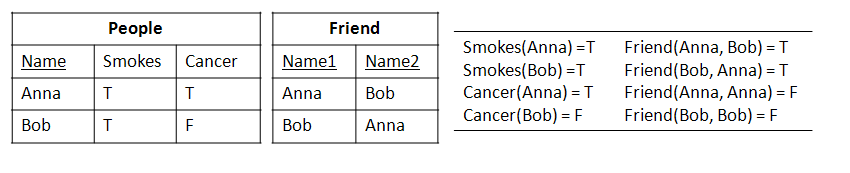
\includegraphics[width = 0.5 \textwidth]{database}
%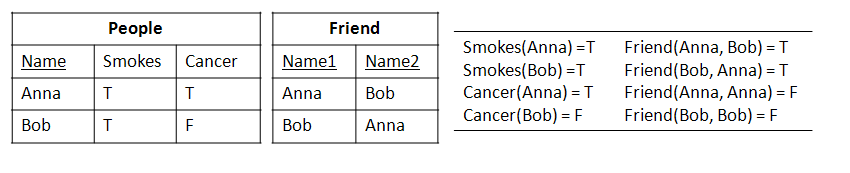
\includegraphics[width=1\textwidth]{database.png}
%}
\caption{A simple relational database instance.
%that are true in the database. 
\label{fig:db-tables}}
\end{center}
\end{figure}


\begin{figure}[t]
\begin{center}
%\resizebox{\textwidth}{!}{
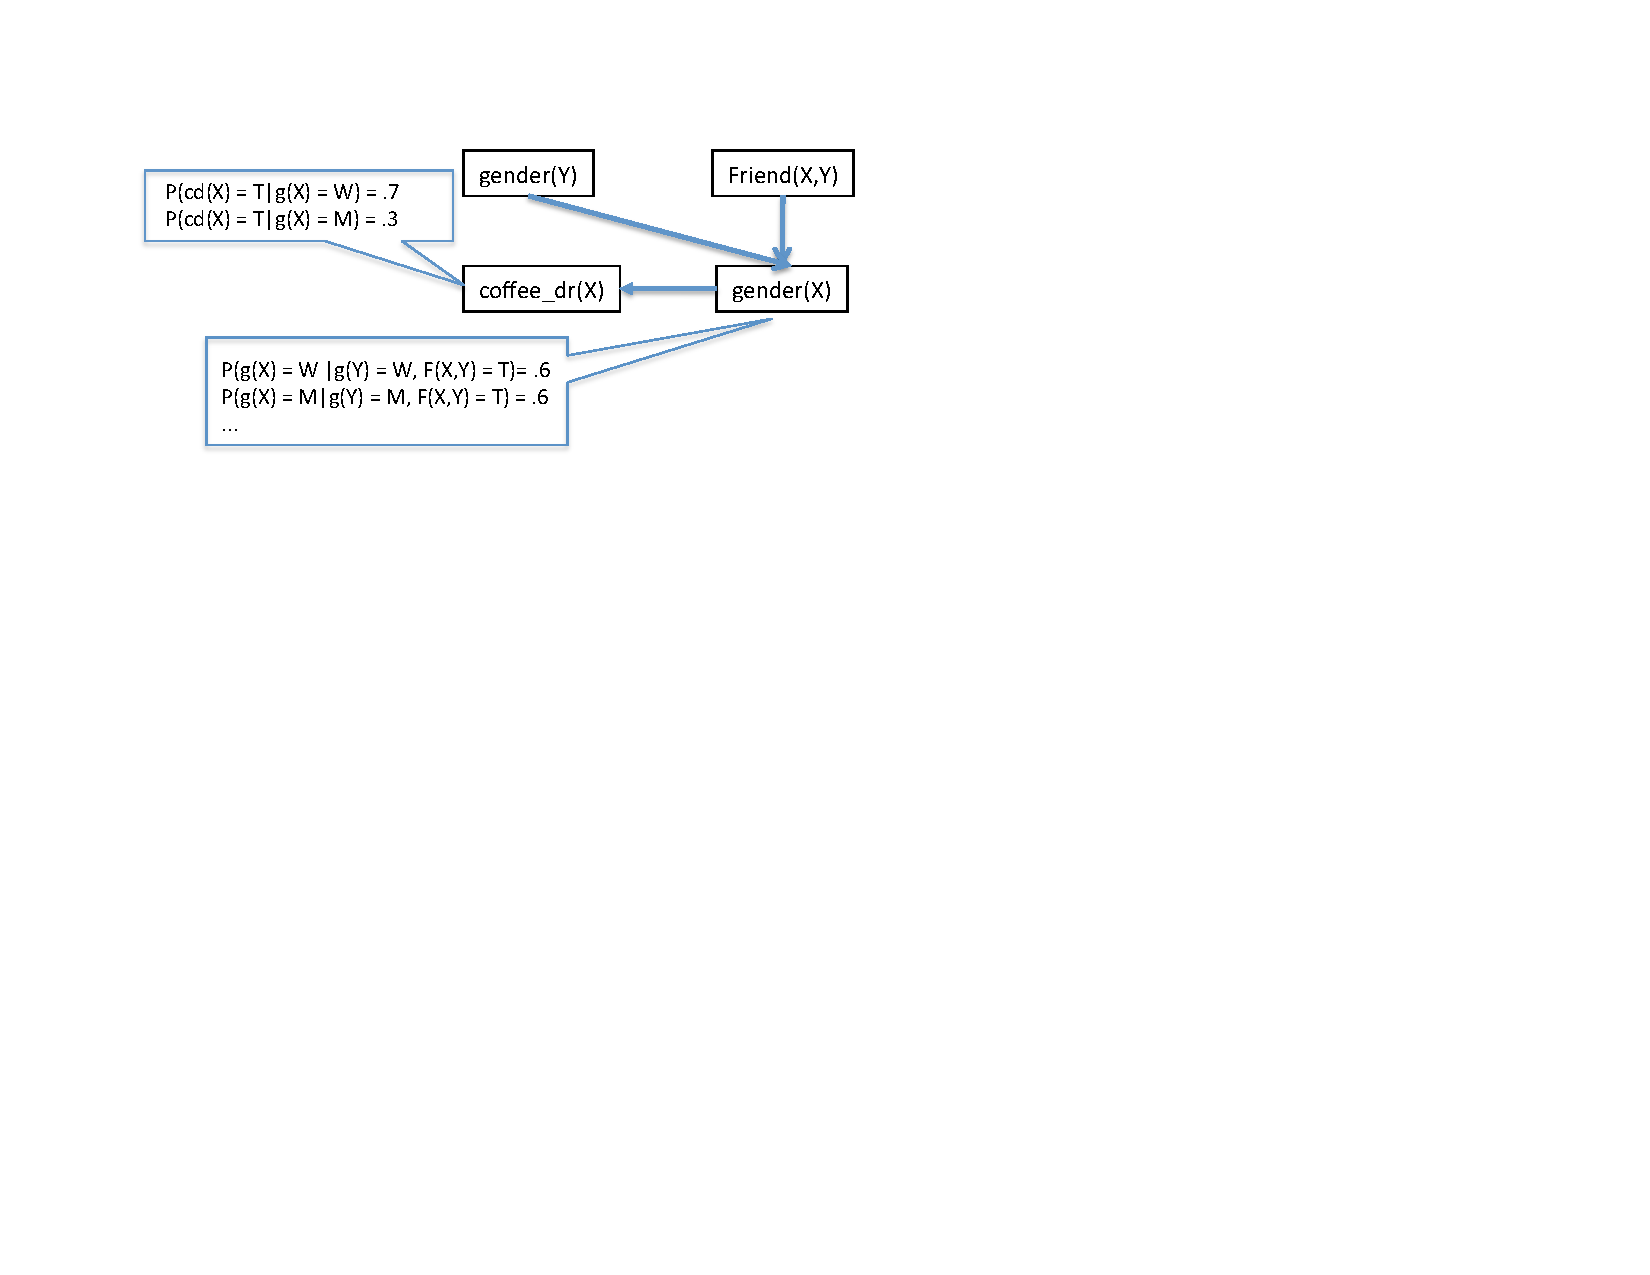
\includegraphics[width = 0.5 \textwidth]{graph-examples}
%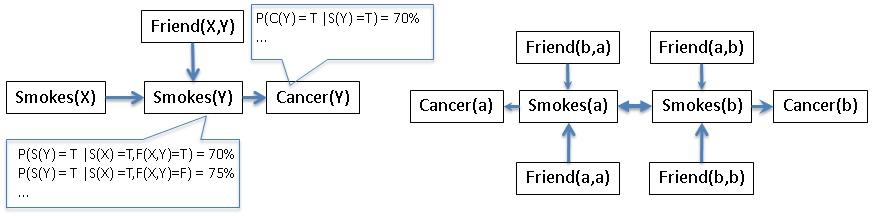
\includegraphics[width=2 \textwidth]{combine1.jpg}
%}
\caption{%A simple relational database instance. 
A Parametrized Bayes Net with some CP-table entries.
 CP-table entries are chosen for illustration and are not related to the data in Figure~\ref{fig:db-tables}. 
For convenience, examples below use a uniform prior over the nodes $\it{gender}(\Y)$ and $\it{Friend}(\X,\Y)$.
\label{fig:pbn}}
\end{center}
\end{figure}

%Recursive dependencies (autocorrelations) are represented in a PBN by ``copies'' of the functors. Thus t
%We assume that the Bayes net is in main functor format \cite{Schulte2012a}: for each functor $\functor$, there is a main functor node that is the only $\functor$-node with parents. In the example, $\it{gender}(\X)$ is the main functor, and $\it{gender}(\Y)$ is an auxilliary functor used only for representing the recursive dependency. 
%The intuition is that since different functor nodes with the same functor are statistically interchangeable, it suffices to select one for modelling the conditional distribution. 
%\footnote{While the existence of a main functor may seem like a strong assumption, Schulte {\em et al.} show that under a mild ordering condition on the BN structure, for every PBN $\B$ not in main functor format, there is an equivalent main functor Bayes net $\B'$ that has the same ground graph \cite{Schulte2012a}.}

\section{Log-linear Relational Regression}

%In this section we consider how the predictor variables $x_{i}$ may be derived from a Bayes net. In the next section we examine how the weight parameters $w_{i}$ may be derived from a Bayes net.
%
%Given a Bayes net model, the $x_{i}$ are derived from the states $\family_{ijk}$ of the Markov blanket of target node $y$. 
Given a PBN, let $\Y = \functor(a_{1},\ldots,a_{\l})$ be a target ground node instantiating functor node $\functor(\A_{1},\ldots,\A_{\l})$.
%\footnote{[If there are several nodes with functor $\functor$, we assume that there is only one node with $\functor$ that has parents, and use that node. Schulte {\em et al.} prove that under a mild ordering condition on the BN structure, for every PBN $\B$ there is an equivalent PBN $\B'$ that satisfies the unique node condition and has the same ground graph \cite{Schulte2012a}.]}
The \textbf{regression graph} for $\Y$ is the partially ground PBN %$B_{Y}$ 
that results by substituting $a_{i}$ for $A_{i}$ in functor node $Y$ {\em and} in its Markov blanket; see Figure~\ref{fig:regress}. A key difference between propositional and relational data is that a Markov blanket state can be instantiated more than once in the relational neighborhood of the target node.
%Recall that 
%the general form of a log-linear regression equation is
%%
%$ln(P(\Y = \y|\set{x}))= \sum_{i} w_{i} x_{i}.
%$
%. This is illustrated in Figure~\ref{fig:regress} for the grounding $\X:= \it{sam}$. 
Accordingly, we consider two choices of predictor variables $\{x_{i}\}$ for lifting the propositional BN local model \eqref{eq:bn-mb} to the relational case: 
%
%\begin{description}
%\item[The Frequency Model] The predictor variables $x_{i}$ are the {\em frequencies} $\prob^{\Y}_{ijk}$.
%% of the Markov blanket states for the target node $\Y$.
%\item[The Count Model] The predictor variables are the {\em counts} $\instances^{\Y}_{ijk}$.
%% of the Markov blanket states for the target node.% $\Y$. 
%\end{description}
%
In the \textbf{frequency model}, the predictor variables $x_{i}$ are the {\em frequencies} $\prob^{\Y}_{ijk}$. In the \textbf{count model},
% of the Markov blanket states for the target node $\Y$.
the predictor variables are the {\em counts} $\instances^{\Y}_{ijk}$.
%
Here and elsewhere the superscript $\Y$ indicates that the notation is used with reference to the regression graph for target node $\Y$. 

If the BN log-conditional probabilities are used as weights, then the
\textbf{count regression equation} is given by 

\begin{equation} \label{eq:regress-count}
ln(P(\Y = \y|\set{X}=\set{x})) = \sum_{ijk} \instances^{\Y}_{ijk} \; ln(\theta_{ijk}) - ln(Z).
\end{equation}

%The summation is over $\Y$'s Markov blanket in the regression graph, so the index $i$ ranges over the target node and its children. 
Equation~\eqref{eq:regress-count} has a straightforward semantics as a grounding of the propositional BN regression equation~\eqref{eq:bn-mb}: After instantiating the regression graph with each possible grounding, apply the BN formula to each ground instance of a conditional probability term.
%; the difference is that a Markov blanket state can have more than one instance for a given target node.
%can be interpreted as instantiating the standard Bayes net regression equation~\eqref{eq:bn-mb}, taking the product of all groundings of Markov blanket probabilities. 
%can be interpreted as instantiating the standard Bayes net regression equation~\eqref{eq:bn-mb}, taking the product of all groundings of Markov blanket probabilities. 
%
The
\textbf{frequency regression equation} is given by 
\begin{equation} \label{eq:regress-frequency}
ln(P(\Y = \y|\set{X}=\set{x})) = \sum_{ijk} p^{\Y}_{ijk} \; ln(\theta_{ijk}) - ln(Z).
\end{equation}

%This equation instantiates the BN Markov as follows. First, for each conditional probability associated with a Markov blanket state, take the geometric mean of the state's groundings. Second, multiply together the geometric means.
Including irrelevant predictors leads to bad predictions, so like other statistical-relational models, we only consider instances that are linked to the target node by some relationship type (i.e., we do not consider negated links). 
Figure~\ref{fig:regress-example} provides example computations.
 %for frequency regression and for count regression. 
 The example illustrates how frequency regression addresses the scale imbalance problem. 

%statistical-relational models restrict edges in the ground model to relevant predictors only \cite{Poole2003}. % add Natarajan on cominbing rules, Getoor and Grant. 
%In what follows, we take the relevance conditions to be the existence of a link, {\em so we only consider instances of the Markov blanket that are related to the target node.} 

\begin{figure}[t]
\begin{center}
%\resizebox{1\textwidth}{!}{
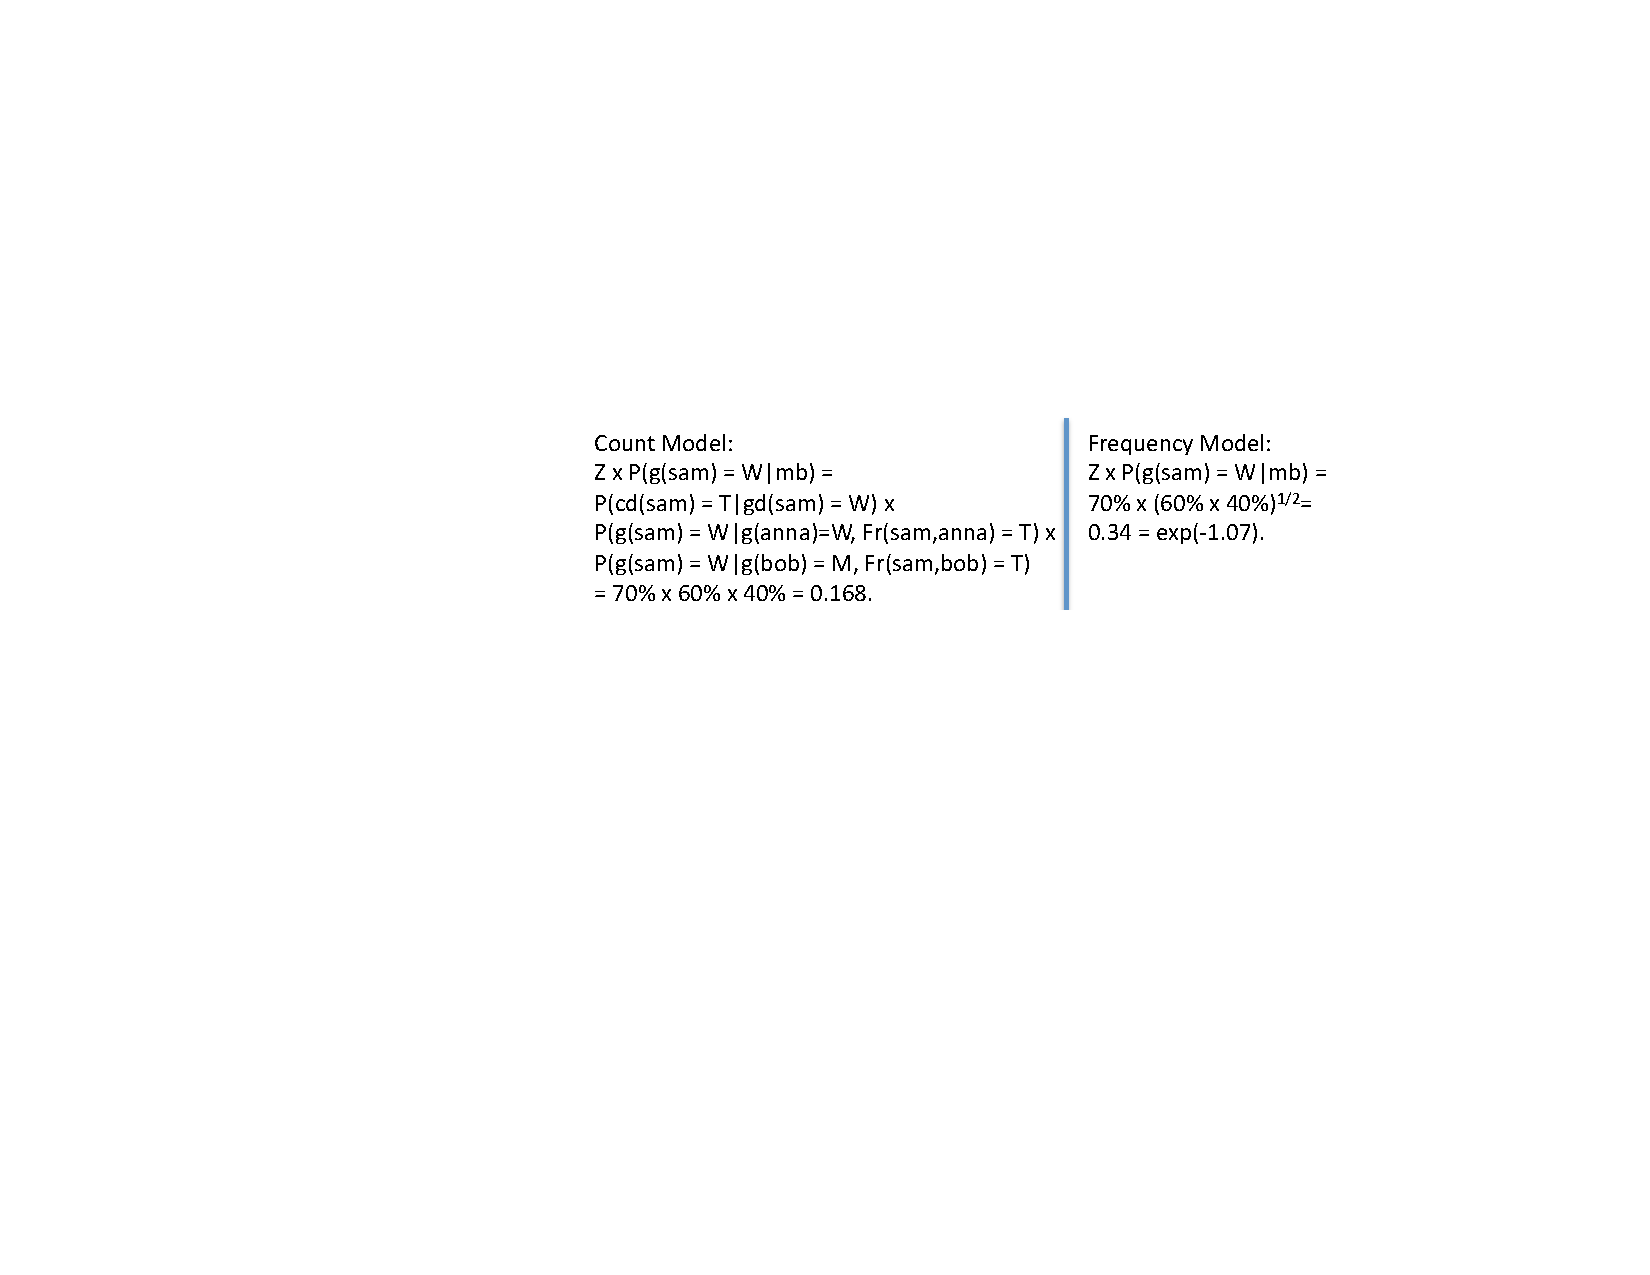
\includegraphics[width=0.5 \textwidth]{regression-example}
%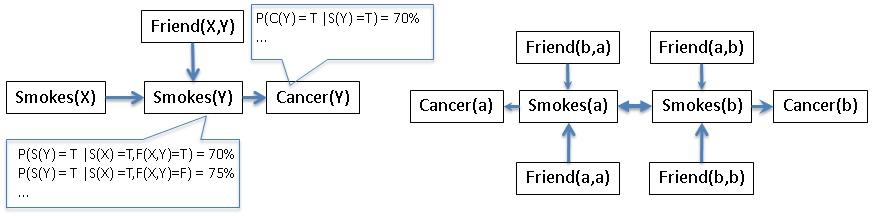
\includegraphics[width=2 \textwidth]{combine1.jpg}
%}
\caption{%A simple relational database instance. 
The computation of the local regression probability for the gender of Sam.
%, for the count model (left) and the frequency model (right). 
%The frequency model assigns higher importance to the factor that represents the coffee drinking of Sam. Notice that the log-probability defined by the frequency models agrees with the log-probability defined by random regression.
 \label{fig:regress-example}}
\end{center}
\end{figure}
The frequency equation sums the log-averages of the groundings of each conditional probability term. We introduce a novel semantics to relate this to the propositional BN local distribution model: Whereas the count equation  results from applying the propositional formula~\eqref{eq:bn-mb} to a {\em complete} grounding of the regression graph, the frequency model results from applying the propositional formula to a {\em random} grounding of the regression graph.

%
%In terms of the ground regression graph, for each child node in the Markov blanket, including the target node, frequency regression takes the geometric mean of the family groundings for that child node, then multiplies together the means. Since this is not a straightforward grounding of the standard BN local product model, we provide an alternative semantics that shows that frequency regression computes the expected value that results from applying the BN regression formula~\eqref{eq:bn-mb} to a random instantiation of the Markov blanket. Thus the count model results from applying the BN product formula to a {\em complete} grounding of the regression graph, whereas the frequency model results from applying the product formula to a {\em random} grounding of the regression graph.


%
%Let $m_{iik}^{\Y}$ denote the number of possible groundings of family formula $\family_{ijk}$. 
%%in the regression graph. 
%Here and elsewhere the superscript $\Y$ indicates that the notation is used with reference to the regression graph. If the parents of functor node $i$ contains a relevance condition,   then $m_{ijk}^{\Y}$ denotes the possible number of relevant groundings. For instance, in the regression graph of Figure~\ref{fig:regress}, $m_{ijk}^{\Y}$ with functor node $i$ being $\it{gender}(sam)$, the term $m_{ijk}^{\Y}$ is the number of Sam's friends. 
%Note that $m_{i}$ does not depend on $j$ or $k$. 
%Then the frequency of the family constellation $\family_{ijk}$ is given by dividing the number of satisfying instantiations by $m_{i}$. 


%\begin{equation} \label{eq:regress-frequency}
%P(\Y = \y|\set{X}=\set{x}) = exp\left(\sum_{ijk} \frac{\instances_{ijk}(\set{X}=\set{x},\Y = \y)}{m_{i}} \cdot ln(\theta_{ijk})\right).
%\end{equation}

%\begin{equation} \label{eq:regress-frequency}
%ln(P(\Y = \y|\set{X}=\set{x})) = \sum_{ijk} \frac{\instances^{\Y}_{ijk}(\set{X}=\set{x},\Y = \y)}{m_{ijk}^{\Y}} ln(\theta_{ijk}).
%\end{equation}



%where $P(\Y = \y|\set{X}=\set{x}))$ is the unnormalized probability of a target node value $\Y = \y$ given an assignment of values to all other nodes. 

%The fraction $\instances^{\Y}_{ijk}/m_{ijk}^{\Y}$ is the number of relevant groundings that satisfy family formula $\family_{ijk}$, divided by the total number of relevant groundings, and therefore represents the frequency of family state $\family_{ijk}$ in the set of relevant groundings.
%that avoids an enumeration of all possible groundings of the Markov blanket.

%
%While random regression sums over all groundings of the Markov blanket, frequency regression sums over the {\em non-ground} functor nodes in the Markov blanket. Thus frequency regression provides an efficient closed-form for computing the random regression value.
%We remark that the equivalence between random and frequency regression holds with any graphical model based on a first-order template, not only Bayes nets. 
%Frequency regression can be interpreted in terms of a dependency network that results from grounding a PBN model: The use of frequency predictors is equivalent to using the {\em geometric mean} to combine conditional probabilities in the Markov blanket of the target node, as Figure~\ref{fig:regress} illustrates.


%Since Equation~\ref{eq:regress-count} uses the family counts $\instances_{ijk}$ rather than the family frequencies $p_{ijk}$, we refer to it as the \textbf{count equation}. 


%\paragraph{Inference.} 
%Assuming complete data, the regression equations can be evaluated in closed-form for conditional inference. We outline how the regression models can be extended to general joint inferences. For the count model, Markov logic network inference algorithms can be used after moralization, as in \cite{Khosravi2012a,Schulte2012}. 
%Heckerman et al. \cite{Heckerman2000} show that applying Gibbs sampling to a dependency network defines a stationary joint distribution, hence can be used to answer general queries based on random/frequency regression. Their ordered pseudo-Gibbs sampler has been lifted to the relational setting \cite{Neville2007}. 
%%A Gibbs sampler for random regression would be able to exploit the ordering constraints provided by the Bayes net structure. 
%Since the form of the frequency equation is very similar to that of the count model, an alternative is to adapt MLN inference methods developed for the count model.
%
%So far we have considered how to derive the predictor variables $x_{i}$ from a given Bayes net graph. 



\section{Random Selection Interpretation.}
%The frequency regression value can be interpreted as an expectation over random instantiations of the Markov blanket as follows.
%We first define random regression, then provide a closed form for computing its value that leads to the frequency log-linear model. The frequency model is a locally scaled version of the standard count log-linear model that is derived from Markov random fields.
%
%\subsection{Definition of Random Regression}
%If there is more than one functor node with $\functor$, we use the main functor node (Sec.~\ref{sec:graph-relational}). 
Given a target node value $\y$ and an assignment $\set{X} = \set{x}$ of values to all ground nodes other than $Y$, random regression is defined by the following steps.
%For an assignment $\set{X} = \set{x}$ of values to all ground nodes other than $Y$, let $\instances_{ijk}(\set{X}=\set{x};\Y=\y)$ be the number of instantiations in the partially ground model that assign value $y$ to $Y$, and whose family state is $\family_{ijk}$. If family $\family_{ijk}$ does not contain functor node $\functor$,  $\instances_{ijk}(\set{X}=\set{x};\Y=\y) = 0$. If the PBN contains more than one node with functor $\functor$, the instances are counted with respect to grounding the main functor node. 

\begin{enumerate}
\item Let $\A_{1},\ldots,\A_{k}$ be a list of {\em all} first-order variables that occur in the Markov blanket of target node $\Y$ in the regression graph for $\Y$.
\item Select an instance (constant) $a_{i}$ from the population of $\A_{i}$, for each $i=1,\ldots,k$; the selections are random, independent, and uniform. Replace each node in the Markov blanket with the corresponding ground node.
\item Using the values assigned to the ground nodes in the database, apply the Bayes net Markov blanket equation~\eqref{eq:bn-mb} 
to compute a log-sum for the random instantiation $\set{a_{i}}$. The {\em expected value} of this log-sum is the \textbf{random regression} value $ln(P^{r}(\Y = \y|\set{X}=\set{x}))$. 
\end{enumerate}

\begin{figure}
\begin{center}
%\resizebox{1\textwidth}{!}{
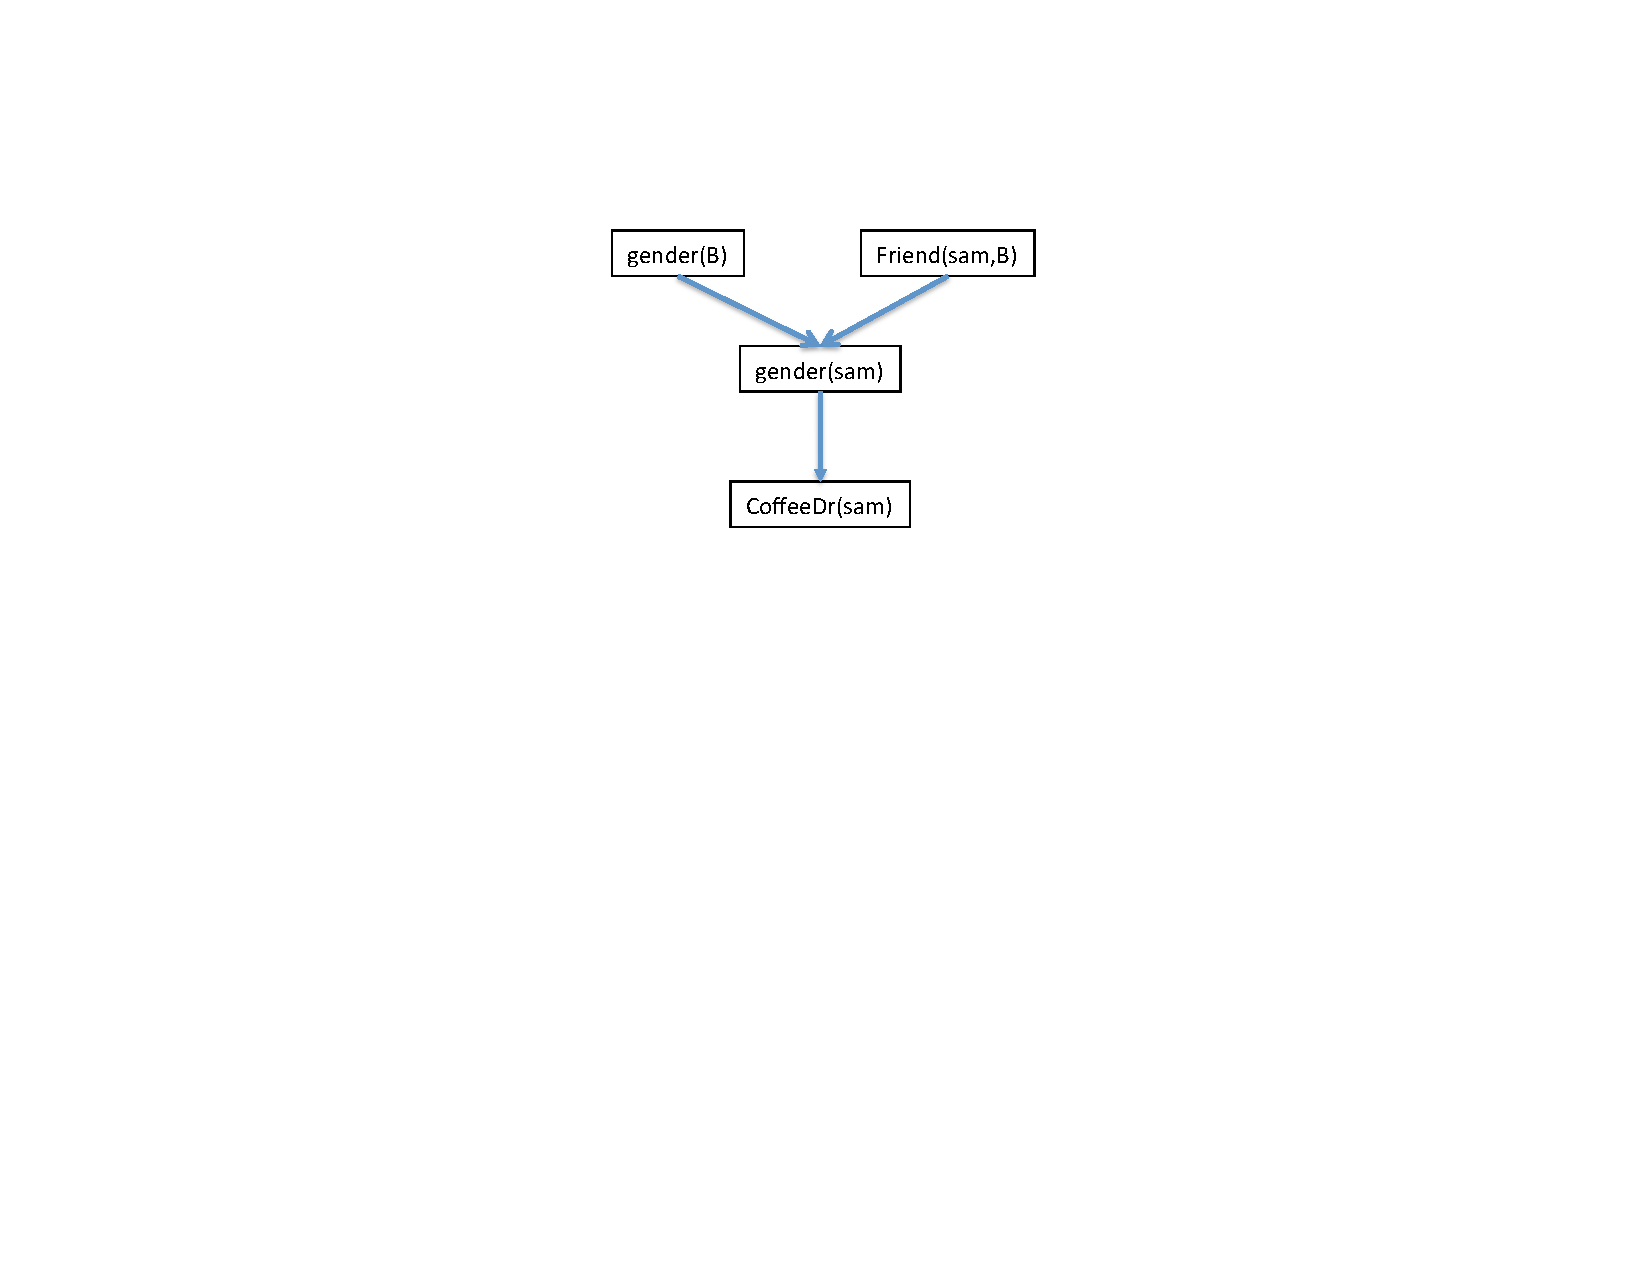
\includegraphics[width =0.3 \textwidth]{regression-graph}
%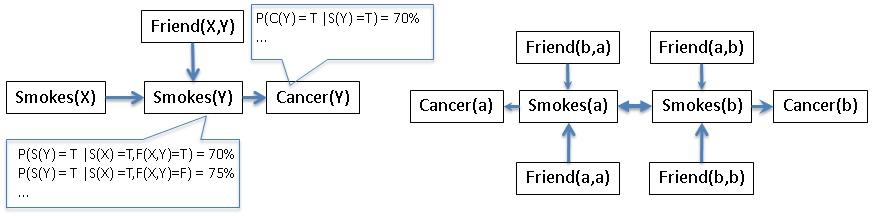
\includegraphics[width=2 \textwidth]{combine1.jpg}
%}
\caption{%A simple relational database instance. 
The regression graph for the target node $\it{gender}(sam)$ derived from the Bayes net of Figure~\ref{fig:pbn} by substituting $sam$ for $\X$.
 \label{fig:regress}}
\end{center}
\end{figure}


 Table~\ref{table:random-regress} provides a sample computation of a random regression for predicting the gender of Sam given the database instance of Figure~\ref{fig:db-tables}. %
%The random regression inference model can be interpreted in terms of a ground dependency network, whose graph structure is given by converting the Bayes net to a dependency network (Sec.~\ref{sec:conversions}), and whose conditional probability parameters are given by random regression. 
%
Applying random regression to $\it{gender}(sam) = W$ (Table~\ref{table:random-regress}) gives the same value as frequency regression, namely $-1.07=ln(0.34)$.
%, conditional on its Markov blanket. 
The next theorem shows that {\em the  equivalence between frequency and random regression holds in all cases.}  The proof is omitted due to space constraints.
\begin{theorem} \label{prop:randomize}
The frequency regression value  for a target node (Equation~\eqref{eq:regress-frequency}) equals the random regression value. 
%; in symbols, $P^{r} = P^{\pseudo}$.
\end{theorem}
%


\begin{table}[htdp]
\caption{Computing the random regression for target node value $\it{gender}(sam) = W$. We use obvious abbreviations for functors. Each friend selection defines an instantiation of the Markov blanket of the target node with two associated factors. %The random regression value -1.07 is the log-average. 
%Notice that $-1.07=ln(0.34)$, the log of frequency regression (Figure~\ref{fig:regress}).
}
\begin{center}
\resizebox{0.5\textwidth}{!}{
  \begin{tabular}{@{} |c|c|c|c| @{}}
    \hline
  Grounding & Factor 1 & Factor 2 & Log-Product \\
    \hline \hline
   $Y=anna$ & \begin{tabular}{@{} l @{}}
$P(\it{cd}(sam) = T|g(sam) = W)$ \\
= .7\\ \end{tabular} & 
\begin{tabular}{@{} l @{}}
    $P(g(sam)=W|g(anna) = W, $ \\ 
    $Fr(sam,anna) = T) = .6$\\ 
  \end{tabular} & 
  \begin{tabular}{@{} l @{}}$ln(.7\times.6)$ \\= -0.87\end{tabular} 
  \\\hline
    Y=bob & \begin{tabular}{@{} l @{}}
$P(\it{cd}(sam) = T|g(sam) = W)$ \\
= .7\\ \end{tabular} & \begin{tabular}{@{} l @{}}
   $P(g(sam)=W|g(bob) = M, $ \\ 
    $Fr(sam,bob) = T) = .4$\\ 
  \end{tabular} & 
  \begin{tabular}{@{} l @{}}$ln(.7\times.4)$ \\=-1.27 \end{tabular} 
  \\\hline
  &  & Average & -1.07 \\ \hline
  \end{tabular}
}
\end{center}
\label{table:random-regress}
\end{table}%


%Figure~\ref{fig:regress} illustrates the resulting computation for predicting the intelligence of Bob given the database instance of Figure~\ref{fig:db-tables}.


%For the relevance version, treat each context sentence as having disjoint variables from the others (e.g. R(X,Y), R1(X1,Y1)). Then you get random selections from contexts.

%\begin{table}[htdp]
%\caption{Computing the random regression for target node node value $\it{gender}(sam)$. Each course selection defines an instantiation of the Markov blanket of the target node with two associated factors. The random regression value -1.07 is the log-average. Notice that $-1.07=ln(0.34)$, the log of frequency regression (Figure~\ref{fig:regress}).}
%\begin{center}
%\resizebox{0.5\textwidth}{!}{
%  \begin{tabular}{@{} |c|c|c|c| @{}}
%    \hline
%  Grounding & Factor 1 & Factor 2 & Log-Product \\
%    \hline \hline
%   $C=100$ & \begin{tabular}{@{} l @{}}
%$P(i(bob) = lo|r(bob) = lo)$ \\
%= .7\\ \end{tabular} & 
%\begin{tabular}{@{} l @{}}
%    �$P(i(bob) = lo|diff(100) = lo, $ \\ 
%    � $R(bob,100) = T) = .6$\\ 
%  \end{tabular} & $ln(.7\times.6)$ = -0.87 \\\hline
%    C=200 & \begin{tabular}{@{} l @{}}
%$P(i(bob) = lo|r(bob) = lo)$ \\
%= .7\\ \end{tabular} & \begin{tabular}{@{} l @{}}
%    �$P(i(bob) = lo|diff(200) = hi, $ \\ 
%    � $R(bob,200) = T) = .4$\\ 
%  \end{tabular} & $ln(.7*.4)=-1.27$ \\ \hline
%  &  & Average & -1.07 \\ \hline
%  \end{tabular}
%}
%\end{center}
%\label{table:random-regress}
%\end{table}%

%Grounding & Factor 1 & Factor 2 & Log-Product \\
%C=100 & P(i(bob) = lo|r(bob) = lo) = .7 & P(i(bob) = lo|diff(100) = lo, R(bob,100) = T) = .6 & -0.87 \\
%C=200 & P(i(bob) = lo|r(bob) = lo) = .7 & P(i(bob) = lo|diff(200) = hi, R(bob,200) = T) =.4 & -1.27 \\
% &  & Average & -1.07 \\

%\subsection{Comparison With Other Log-Linear Models} 
%
%\label{sec:conversions}
%
%
%A \textbf{Markov network} structure is an undirected graph. For each clique $\clique$ in the graph, 
%a \textbf{clique potential function} $\potential_{\clique}$ specifies a nonnegative real number for each possible assignment of values to the clique. 
%%For an assignment of values to all nodes in the Markov net, the joint probability of the values is given by the product of the associated clique potentials, divided by a normalization constant.
%
%A \textbf{dependency network} structure is a directed graph; cycles are allowed \cite{Heckerman2000,bib:jensen-chapter,Natarajan2012}. 
%The parameters are conditional probabilities of each node, given its {\em Markov blanket}.
% %(not just the parents).  
%% Dependency networks are like Markov networks, in that conditional probabilistic independence corresponds to graph separation. They are like Bayes nets, in that the parameters are conditional probabilities.
%
%
%A Bayes net can be converted to a Markov net through the standard \textbf{moralization} method: connect all co-parents, and make all edges in the resulting graph undirected. Thus each family in the Bayes net becomes a clique in the moralized structure. For each state of each family clique, we define the clique potential in the Markov net to be the conditional probability of the child given its parents. 
%%This is the conversion procedure recommended by Domingos and Richardson \cite{Domingos2007} and by the Alchemy group \cite{bib:bayes-convert}.
%%The resulting Markov net defines the same joint probability over assignments of values to the nodes as the original Bayes net. 
%%If $M(\B)$ is a Parametrized Markov net obtained from PBN $B$, the unnormalized likelihood function for the ground graph of $M(\B)$ \cite{Domingos2009} is given by
%%
%%\begin{equation}\label{eq:mbn-likelihood}
%%    P_{\M(\B)}(\set{V} = \set{v}) = exp\left(\sum_{ijk} \instances_{ijk} \cdot ln(\theta_{ijk})\right).
%%\end{equation}
%
%%This is because each ground parent-child instance corresponds to a conditional probability $\theta_{ijk}$, viewed as a clique potential, so 
%%Thus the likelihood is proportional to the product of all conditional probabilities. 
%%In terms of the Bayes net parameters, Equation~\eqref{eq:mbn-likelihood} is simply the product of all conditional probabilities defined by a ground child-parent instance.
%A PBN graph can be converted to a Markov Logic Network structure by moralization \cite[12.5.3]{Domingos2007}, \cite{Schulte2012}: for each family state $\family_{ijk}$, add a conjunction of literals that specifies the state.
%
%
%Bayes nets can also be converted to dependency nets \cite{Heckerman2000}. For each node $\X_{i}$, and each node  $\X_{j}$ in the Markov blanket of $\X_{i}$, add a directed edge $\X_{j} \rightarrow \X_{i}$. 
%%The resulting graph is the same as the moralized Bayes net structure but with bidrected rather than undirected adjacencies. 
%The conditional probability parameters are  given by the Markov blanket equation ~\eqref{eq:bn-mb}.
%
%%A \textbf{Markov Logic Network} (MLN) is a finite set of 1st-order formulas or clauses $\{\formula_{i}\}$, where each formula $\formula_{i}$ is assigned a weight. 
%%A Markov Logic Network can be viewed as a specification of a Markov network using logical syntax \cite{Domingos2009}. Given an MLN and a database $\D$, let $n_{i}(\D)$ be the number of groundings that satisfy $\formula_{i}$ in $\D$.
%%%An MLN assigns a log-likelihood to a database according to the equation
%%%
%%%\begin{equation}\label{eq:log-linear}
%%%ln(P(\D)) = \sum_{i} w_{i} n_{i}(\D) - ln(\Z)
%%%\end{equation}
%%%where $\Z$ is a normalization constant.
%%%
%%%Thus the log-likelihood is a weighted sum of the number of groundings for each clause. 
%%
%%Functor Markov Nets have a simple representation as Markov Logic Networks as follows. For each assignment of values to a clique of functor nodes, add a conjunctive formula to the MLN that specifies that assignment. The weight of this formula is the logarithm of the clique potential. For any Functor Markov net,  the MLN likelihood function defined by Equation~\eqref{eq:log-linear} for the corresponding MLN is exactly the Markov net likelihood defined by grounding the Functor Markov net. {\em Therefore we can use MLN inference to carry out inference for Functor Markov Nets.}
%
%The count equation is closely related to Markov random fields, as follows. Consider the Parametrized Markov net $M$ obtained by moralizing the PBN (Sec.~\ref{sec:conversions}). The count equation follows from applying the standard Markov field regression equation to the grounding of $M$ \cite{Domingos2007}. 
%%In graphical terms, the equation is the product of all clique potentials in which the target node participates; see Figure~\ref{fig:regress-example}. 
%%Count regression is a natural comparison point to random regression due to their similarity. 
%%
%%In the count regression equation~\eqref{eq:regress-count}, Markov blanket components with many groundings have exponentially more influence. 
%%In a typical scenario, a descriptive attribute of a target entity corresponds to a single factor, whereas the attributes of related entities correspond to many, as many as there are related entities. For example, in the prediction of intelligence in Figure~\ref{fig:regress}, the factors due to courses quickly overwhelm the influence of rank as the number of courses increases. 
%%The frequency model balances the scales of the predictor variables, such that their common range is [0,1]. 
%In terms of the factor products defined by exponentiating the log-linear equations, the two models compare as follows. The count equation multiplies together all ground Markov blanket factors, whereas the frequency equation first computes the {\em geometric mean} of the ground factors associated with each functor node in the Markov blanket, then multiplies these geometric means (Figure~\ref{fig:regress-example}). Both regression models can be interpreted in terms of a dependency network that results from grounding a PBN model.
%Figure~\ref{fig:derivations} summarizes the connections between graphical models and regression equations. In the next section we consider how to derive the weight parameters from given Bayes net parameters.
%
%\begin{figure}[htbp]
%\begin{center}
%%\resizebox{0.5\textwidth}{!}{
%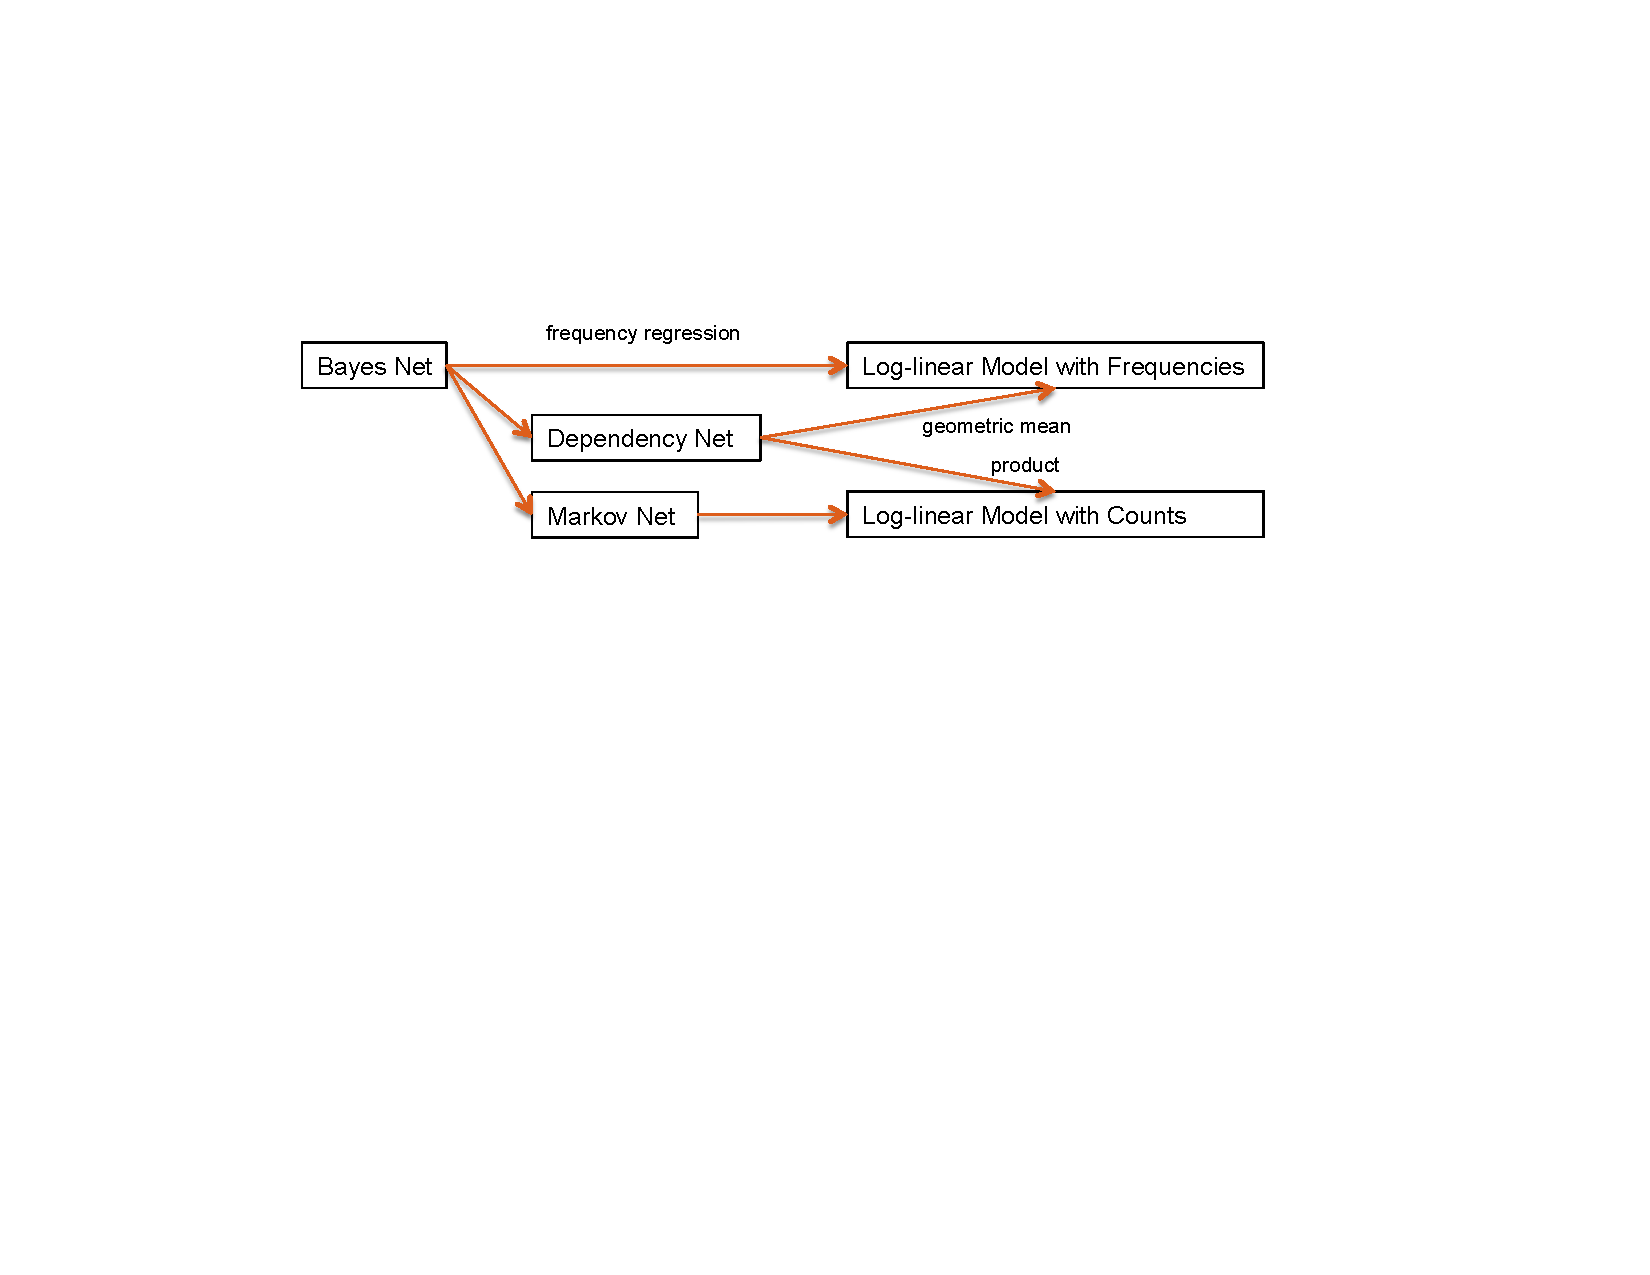
\includegraphics[width = 0.5 \textwidth]{derivations}
%%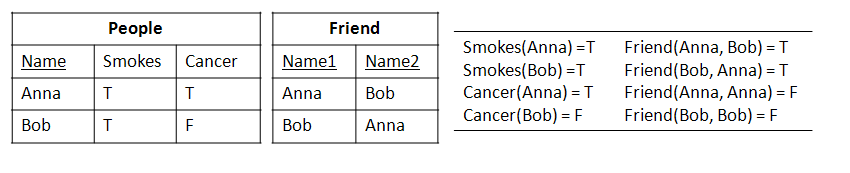
\includegraphics[width=1\textwidth]{database.png}
%%}
%\caption{Connections between graphical models and log-linear regression equations. 
%%Applying random regression directly to a PBN leads to the frequency model (Theorem~\ref{prop:randomize}). Converting the Bayes net to a Markov net leads to the count model. Converting the Bayes net to a dependency network leads to the frequency model if the geometric mean is used to combine Markov blanket conditional probabilities. Using the product of conditional probabilities instead leads to the count model. 
%\label{fig:derivations}}
%\end{center}
%\end{figure}
%
%
%\section{Weight Learning With Bayes Net Parameters}
%
%For estimating the conditional probabilities, we use the empirical conditional frequencies observed in the database:
%
%\begin{equation*} \label{eq:frequencies}
%\widehat{\theta}_{ijk}(\set{V} = \set{v}) = \frac{n^{\Y}_{ijk}(\set{V} = \set{v})}{\sum_{k}n^{\Y}_{ijk}(\set{V} = \set{v})}.
%\end{equation*}
%
%These estimates are well motivated by the following theoretical and practical considerations. 
%%\marginpar{check Poole}
%
%\emph{Maximum Likelihood.} The  random selection pseudo-likelihood for a Bayes net is the natural generative counterpart of random regression \cite{Schulte2011}. This measure is the expected log-likelihood of a random instantiation of all first-order variables in the Bayes net. The pseudo-likelihood is maximized by the conditional frequencies $\widehat{\theta}_{ijk}$ in the database \cite[Prop.3.1]{Schulte2011}. 
%%This result is a counterpart to the standard maximum likelihood solution for i.i.d. propositional data.
%
%\emph{Interpretability.} The weight/clique potential parameters of undirected models are often difficult to interpret for users \cite{Pearl1988}. 
%This is especially the case when weights are learned from data, with complex interactions between weights assigned to different local cliques. In contrast, a Bayes net parameter can be interpreted as a conditional probability, and reflects local statistics restricted to a parent-child constellation.
%
%\emph{Scalability.} 
%Using frequency estimates can be viewed as a type of {\em lifted learning}, by which we mean using only the sufficient statistics in a relational database, rather than an iteration over ground facts. The computational cost of lifted learning scales well in both data size and the number of parameters in the model. 
%%
%We investigate two methods for converting Bayes net conditional probabilities to log-linear weights $w_{ijk}$. 
%
%\subsection{Log-conditional Probabilities as Weights.} \label{sec:logprob} The first method uses the logarithm of the conditional probability of a child node value given values for its parents. In symbols:
%
%\begin{equation*}
%w_{ijk} := ln(\theta_{ijk}).
%\end{equation*}
%
%{\em Example.} As in Section~\ref{sec:graph-relational}, consider the family state 
%$\family_{ijk}$ with $\theta_{ijk} = 40\%$. In the Markov Logic network that results from converting the PBN, this parameter leads to the weighted conjunctive clause 
%\[g(\X)= M, g(\Y) = W, F(\X,\Y) = \true; w = ln(40\%).\]% = -0.916. \]
%
%Other researchers have recommended log-conditional probabilities as weights   \cite{Domingos2007}, \cite{bib:bayes-convert}. 
%In the propositional case, if we convert a Bayes net to a Markov net by moralization and use the log-conditional probabilities as weights (logarithm of clique potentials), then the joint distribution defined by the Bayes net is equivalent to the joint distribution defined by the Markov net \cite{Lauritzen1996}. 
%
%{\em The Scale Problem.} 
%A problem with using log-conditional probabilities together with the count model is that features with more instances have exponentially more influence; see Figure~\ref{fig:regress-example}. In a typical illustrative scenario, the regression target is the descriptive attribute of a single entity, (e.g., $\it{gender}(sam)$). One predictor feature represents an association between attributes of the same entity (e.g., $\it{coffee\_dr}(sam),\it{gender}(sam)$, whereas another represents an association between attributes of related entities and the single entity (e.g., $\it{gender}(sam), \it{gender}(\Y),\it{Friend}(\it{sam},\Y) = \true$). In this case the information from related entities has many instances, and tends to overwhelm that from the target entity, which has just one instance. In terms of a log-linear model, the count predictors are on different scales. 
%%In a general log-linear model, the weights can be adjusted so that predictors with large values receive smaller weights. But 
%%since in a Bayes net model, the weights are on the same scale (log-probability), log-conditional probabilities do not sufficiently scale down the impact of predictors with larger grounding counts. 
%{\em Frequency regression balances the impact of different features by scaling predictors to the common range [0,1].}  
%Our second conversion procedure also addresses the scale problem,  by adjusting the weights. % derived from log-conditional probabilities.
%
%\subsection{Log-differences as Weights.} 
%\label{sec:log-diff}
%The second method uses the log-difference between the conditional probability of a child node value given values for its parents, and the prior unconditional probability of the child node value. 
%%Recall from Section~\ref{sec:graph-relational} that the notation $\family_{i0k}$ refers to node $i$ taking on value $k$ without any specification of parent values, with the corresponding interpretation of $\instances_{i0k}$ and $\prob_{i0k}$.
%%of the Bayes net parameters as weights. To define this formally, let us first write $\instances_{i0k}(\set{V} = \set{v})$ for the number of groundings of child node $\Y$ such that the ground node $\y$ is assigned value $k$, and similarly $p_{i0k}(\set{V} = \set{v})$ for the frequency of such groundings. 
%A Bayes net implicitly defines a value $\theta_{i0k}$ for the marginal probability of node $\X_{i}$ taking on value $k$, which can be computed using a standard Bayes net query (or directly estimated from the data).
%%If we use maximum likelihood estimation, the empirical frequency of functor node $i$ taking on value $k$ is given by
%%
%%\[\widehat{\theta}_{i0k}(\set{V} = \set{v}) = \frac{\instances_{i0k}(\set{V} = \set{v})}{\sum_{k} \instances_{i0k}(\set{V} = \set{v})}.\]
%%
%The log-difference weight assignment is 
%\begin{equation*}
%w_{ijk} := ln(\theta_{ijk}) - ln(\theta_{i0k}).
%\end{equation*}
%
%%This method requires adding the predictor variable $\instances^{\Y}_{i0k}$ to the count equation~\ref{eq:regress-count}, and the predictor variable $p_{i0k}$ to the frequency equation~\ref{eq:regress-frequency}. In either case, the weight of the new predictor variable is $w_{i0k}$.
%% When discussing the log-difference model, we assume  implicitly that these predictors have been added to the model. In terms of 
%%%Markov random fields, the predictor variables correspond to a potential for a singleton clique; in terms of 
%%Markov Logic Networks, they correspond to adding unit clauses. 
%%
%{\em Example.} For the Bayes net of Figure~\ref{fig:pbn}, assume that conditional on $\X$ and $\Y$ {\em not} being friends, the distribution of $g(\X)$ is  uniform regardless of the value of $g(\Y)$. For instance, $P(g(\X)=W|F(\X,\Y) = F, g(\Y) = M) = 1/2$. Then the marginal probability distribution that the Bayes net entails for $g(\X)$ is also uniform, that is, $P(g(\X) = M) = P(g(\X) = W) = 50\%.$
%%
%For each marginal probability assignment, the Markov Logic network that results from converting the PBN contains a unit clause with weight the log-marginal probability. In the example, there is a weighted clause \[g(\X) = M; w = ln(50\%). \]
%%= -0.693.\] 
%For each family state $\family_{ijk}$, the MLN contains a conjunctive clause, with the weight being the log-difference between the conditional and the marginal probabilities. In the example, there is a weighted clause 
%
%\begin{small}
%\[g(\X)= M, g(\Y) = W, F(\X,\Y) = \true; w = ln(40\%) - ln(50\%).\]
%% = -0.223.\]
%\end{small}
%{\em Motivation and Discussion.} 
%%One advantage of the log-difference method is that the weights can be interpreted in terms of relevance, as usual in a linear model. Thus a positive weight means positive relevance: the parent condition lifts the probability of a child node value, a negative weight means negative relevance: the parent condition lowers the probability of a child node value, and a 0 weight means irrelevance: the parent condition does not affect the probability of a child node value.
%%
%%Our main motivation for the log-difference method is to improve predictions by addressing the scale problem. 
%%For a child node that refers to a descriptive attribute of a single entity, (e.g., $\it{gender}(\X)$), formulas with many groundings are those that express an association between attributes of related entities and the single entity (e.g., the formula $\it{gender}(\Y) = W, \it{gender}(\X)= M,\it{Friend}(\X,\Y) = \true$ introduces a connection between the gender of a user and that of his or her friends). 
%The reason why log-difference addresses the scale problem is as follows.
%Compared to associations among the attributes of a single entity, we expect the associations with related entities to be relatively weak, because probabilistic dependencies in a network become weaker with distance. This means that the probability of a child value, given a parent condition specifying descriptive attributes of related entities, should be relatively close to the marginal probabilities of the child value. Therefore the log-difference should be relatively small, and so the log-difference method tends to assign smaller weights to formulas with many groundings. The supplementary material confirms this expectation with direct observations of the weight sizes assigned to different formulas. It also shows that weights found by Markov field optimization methods are smaller for formulas with many groundings, which is further evidence that a scaling component is important for weights in the count model.
%
%%In the next section we present empirical observations that compare the balancing effect of the log-difference and other weight learning methods.
%
%%
%
%%While using the frequency model is the most direct and effective way to address the scale problem, the log-difference method is useful if the goal is to use a count-based model of inference, such as a Markov Logic Network.
%%We evaluate different weight learning methods in two ways: i) by considering how they scale weights, and ii) by the predictive performance of the resulting models. 
%%
Our experiments evaluate the different methods on learning time and predictive accuracy.

\section{Empirical Evaluation}
We performed extensive experiments; due to space constraints, we describe some key findings and summarize others.
All experiments were done on a QUAD CPU Q6700 with a 2.66GHz CPU and 8GB of RAM. Our code and datasets are available on the world-wide web (reference omitted for blind review).
 %\cite{bib:jbnsite}. 

% and the comparison results.
%\subsection{Datasets}


\subsection{Comparison Methods.}

\subsubsection{Structure Learning.} The learn-and-join algorithm is the state-of-the-art Bayes net structure learning algorithm for relational data \cite{Schulte2012}. To obtain a Bayes net structure, we applied the learn-and-join algorithm to each database.
%, which takes at most 2 minutes on the benchmark databases. %, which is the start of the art structure learning algorithm for Parametrized Bayes Nets 
%
%We then convert the PBN graph to a Markov Logic Network structure (see Section~\ref{sec:conversions}),
%%which adds a conjunctive clause for each family state $\family_{ijk}$ (Section). 
%declaring attribute predicates as functional, as recommended by the Alchemy Group \cite{bib:bayes-convert}. 
%A limitation of the current learn-and-join algorithm is that it learns a generative model over attributes given link structure, so our evaluation considers only queries that target attributes, not links, following \cite{Khosravi2010,Schulte2012}. 

\subsubsection{Parameter Learning.} For estimating BN conditional probabilities, we use the empirical conditional frequencies observed in the database:

\begin{equation*} \label{eq:frequencies}
\widehat{\theta}_{ijk}(\set{V} = \set{v}) = \frac{n^{\Y}_{ijk}(\set{V} = \set{v})}{\sum_{k}n^{\Y}_{ijk}(\set{V} = \set{v})}.
\end{equation*}

A general log-linear model uses weights $w_{ijk}$ in place of $ln(\theta_{ijk})$.
%in place of $ln(\theta_{ijk})$ derived from a conditional probability. 
To learn the $w_{ijk}$ weights, we applied the default weight training procedure of the Alchemy package \cite{Kok2009a} using the same moralization procedure as in \cite[12.5.3]{Domingos2007}, \cite{Schulte2012}: convert a parametrized BN to an MLN structure that contains,  for each family state $\family_{ijk}$ in the BN, a conjunction of literals that specifies the state. It is readily seen that the regression equation for the resulting MLN is the count equation \cite{Schulte2011}. Thus weights learned by Alchemy can be used for count regression. Our comparison methods are the following.
%
%\footnote{In not yet published work, Khosravi proposed computing regression weights by subtracting the logarithm of the uniform distribution over child node values from the conditional probability BN parameters. Empirically we found that the frequency model performs better. Theoretically it can be shown that the frequency model already incorporates a prior term, in that it is equivalent to computing regression weights by subtracting the logarithm of the child node's prior distribution from the conditional probability BN parameters and adding unit clauses for each node. Therefore prior subtraction appears both theoretically and empirically inferior to the frequency model.}
% %(i.e., $ln(1/l)$ for a child node with $l$ possible values)  
% This method is not theoretically equivalent to random regression. We found that using the marginal probabilities $\theta_{i0k}$ performs better than the uniform distribution on both accuracy and log-likelihood. Thus the marginal probabilities appear to be preferable both in terms of theoretical justification and in terms of predictive performance.} 
%\footnote{We also added unit clauses for each node-value combination, as recommended by the Alchemy group.}  
%We refer to this method as the \textbf{MBN} method, for ``Moralized Bayes Net''   \cite{Khosravi2010}. 
%MBN is the state-of-the-art method for log-linear prediction with Bayes nets \cite{Schulte2012}.

\begin{description}
\item[MBN] Converts the Bayes net structure to an MLN using moralization. Learns weights using Markov net methods \cite{Lowd2007}. Uses count regression for inference.
%\item[MBN+Frequency] Same as the previous method, but using frequency regression for inference. 
%Alchemy optimizes weights for the count model; we include this method to assess the impact of frequency scaling for weights other than log-conditional probabilities.
\item[CP+Count]  Parametrizes the Bayes net with the empirical conditional probabilities and uses count regression for inference.
% Actually, this is using the linear shift, or log-difference method.
\item[CP+Frequency]  Parametrizes the Bayes net with the empirical conditional probabilities and uses frequency regression.
\end{description}

% KEEP THIS: if we restrict to relevant relations, we can do the same proof conditional on the existence of a relationship. the only issue is if there are 0 groundings for all applicable formulas. In this case it's better to use log-diff, i.e., the true prior, rather than the uniform one.
%\subsubsection{Inference}
%is performed by evaluating the count resp. frequency regression equation. 

%For MBN we use the count inference model because Alchemy weight learning is optimized for this.
%\footnote{We also experimented with MBN+ the frequency model, with very similar performance to the count model.} 

%
%We compared the following approaches.
%
%
%%\textbf{MLN+ MLN}: We use Alchemy's default program (version x) for producing a parametrized Markov network.
%
%\begin{description}
%\item[MBN] As described above, the Bayes net structure is converted to an MLN using moralization, 
%%\item[MBN+Frequency] Same as the previous method, but using frequency regression for inference. 
%%Alchemy optimizes weights for the count model; we include this method to assess the impact of frequency scaling for weights other than log-conditional probabilities.
%
%\item[CP+Count]  Parametrizes the Bayes net with the empirical conditional probabilities and uses count regression.
%% Actually, this is using the linear shift, or log-difference method.
%\item[CP+Frequency]  Parametrizes the Bayes net with the empirical conditional probabilities and uses frequency regression.
%\end{description}

%We also report results using the recent MLN-Boost learning algorithm \cite{Khot2011}, which is a state-of-the-art learner for undirected relational models. 


We employ exact inference rather than approximate inference (e.g., MC-SAT) to avoid conflating the impact of the model choice with the impact of the inference implementation. We conducted experiments with MC-SAT and the results were similar. 

\subsection{Performance Metrics.}
We use 3 performance metrics: %measures: goo	ggg
Learning Time, Accuracy (ACC), and Conditional Log Likelihood (CLL). ACC and CLL have been used in previous studies of MLN learning  \cite{Domingos2007,Schulte2012}. The CLL of a ground atom in a database is given by the log of the regression equation. For a database we report the average CLL over all atoms in the test set, and the standard deviation. To define accuracy, we apply inference to predict the probability of an attribute value, and score the prediction as correct if the most probable value is the true one. For ACC and CLL the values we report are averages over all predicates that represent descriptive attributes. 
%We do not use Area Under Curve(AUC) as it is mostly used for binary predicates.
%The AUC curves were computed by changing the CLL threshold above which a ground atom is predicted true (10 thresholds were used).
We do not use Area Under Curve, as it mainly applies to binary values, and most of the attributes in our dataset are nonbinary. 
%Like previous studies, we used the MC-SAT inference algorithm \cite{Poon2006} to compute a probability estimate for each possible value of a descriptive attribute for a given object or tuple of objects.  %In principle, our 
We evaluate the learning methods using 5-fold cross-validation as follows. We formed 5 subdatabases for each database, by randomly selecting entities from each entity table, and restricting the relationship tuples in each subdatabase to those that involve only the selected entities  (i.e., subgraph sampling \cite{Frank1977,Schulte2012}). The models were trained on 4 of the 5 subdatabases, then tested on the remaining fold. 
%We report the  average score over the 5 runs, one for each fold. 

\subsection{Databases.}

We used %one synthetic and 
5 benchmark real-world databases.   
%The databases are fairly complex, so the experiments are computationally demanding, especially the Alchemy inference component, which needs to be applied to all groundings of all descriptive attributes to compute average predictive performance. The databases and their main characteristics are as follows. 
For more details please see the references in \cite{Schulte2012}.
% and on-line sources such as \cite{bib:jbnsite}.
%In this paper we report the average result over all subdatabases in this paper and leave the evaluation of how models should evolve based on the size of data to an extension of the work in a journal paper. 


%{\em University Database.} We manually created a small dataset, based on the schema given in Table~\ref{table:university-schema}.
%The dataset is small and is used as a toy example for testing purposes. There are three entity tables, Student, Course, Professor, and 2 relationship tables RA and Registered.
%The entity tables contain 38 students, 10 courses, and 6  Professors. The $\reg$ table has 92 rows and the $\it{RA}$ table has 25 rows. %This dataset is translated into 513 ground atoms.

{\em MovieLens Database.} This is a standard dataset from the UC Irvine machine learning repository. 
% \cite{Schulte2012}.
%The schema for the dataset is shown in Table \ref{}.
%It contains two entity tables: $\it{User}$ and with 941 tuples and $\it{Item}$ with 1,682 tuples, and one relationship table $\it{Rated}$ with 80,000 ratings. The $\it{User}$ table has key field $\it{user\_id}$ and 3 descriptive attributes $\age, \it{gender}, \it{occupation}$. We discretized the attribute age into three bins with equal frequency. The table $\it{Item}$ represents information about the movies. It has 17 Boolean attributes that indicate the genres of a given movie. We performed a preliminary data analysis and omitted genres that have only weak correlations with the rating or user attributes, leaving a total of three genres.
%
%The full dataset contains 170,143 ground atoms and is too big for Alchemy to perform learning. We made small subsamples to make the experiments feasible. Subsampling 100 Users and 100 Items transforms to an Alchemy input file with 3,485 ground atoms. Structure learning with Alchemy takes around 30 min.
%Subsampling 300 Users and 300 Items transforms to an Alchemy input file with 27,134 ground atoms. Structure learning with Alchemy takes about 2 days to run.
%The full table with 100,000 ratings exceeded the memory limits of Tetrad, so we randomly picked 40\% of the ratings of the relationship table as input data.

{\em Mutagenesis Database.} This dataset is widely used in ILP research.
% \cite{Srinivasan1996}. %It contains 4 tables total to 15218 tuples. 
It contains information on Atoms, Molecules, and Bonds between them. We use the discretization of \cite{Schulte2012}.
%
%Mutagenesis has two entity tables, $\it{Atom}$ with 3 descriptive attributes, and $\it{Mole}$, with 188 entries and 5 descriptive attributes, including two attributes that are discretized into ten values each (logp and lumo).
%% There are two relationships $\it{MoleAtom}$ indicating which atoms are parts of which molecules, and $\it{Bond}$ which relates two atoms and has 1 descriptive attribute. 
%The full dataset, with 35,973 ground atoms, crashed Alchemy with both structure  and parameter learning. A subsample with 5,017 ground atoms did not terminate for structure learning, but weight learning was feasible. The computational difficulties of Alchemy compared to the MovieLens dataset are  due to the high number of descriptive attributes.
%%another subsample with
%Representing a relationship between entities from the same table in a parametrized Bayes net requires using two or more variables associated with the same population (e.g., $\it{Bond}(\A_{1},\A_{2}))$.
%(Techreport 2009) describes a straightforward extension of Algorithm~\ref{alg:structure} for this case, which we applied to the Mutagenesis dataset.\footnote{Reference omitted for blind review.}
%We also tested our method on the Financial dataset with similar results, but omit a discussion due to space constraints.

{\em Hepatitis Database.} This data is a modified version of the PKDD02 Discovery Challenge database.
% \cite{Frank2007}. %, which includes removing tests with null values. 
The database contains information on the laboratory examinations of hepatitis B and C infected patients. 
%The examinations were realized between 1982 and 2001 on 771 patients. The data are organized in 7 tables (4 entity tables,  3 relationship tables and 16 descriptive attributes). They contain basic information about the patients, results of biopsy, information on interferon therapy, results of out-hospital examinations, results of in-hospital examinations. 


{\em Mondial Database.} 
%
%\textbf{Hassan: which version did you use? The full one from http://www.dbis.informatik.uni-goettingen.de/Mondial/mondial-ER.pdf or Bahareh's?} 
%
This dataset contains data from multiple geographical web data sources. %Our dataset contains 4 entity tables, $\it{Country},\it{Continent},\it{Economy},\it{Government}$, where the latter three are related to Country by many-one relationships, and one relationship table $\it{Borders}$ that relates two countries.

%Table~\ref{table:datasetsize} lists the resulting full database  sizes in terms of total number of tuples and number of ground atoms, which is the input format for Alchemy. 
%\begin{table}[thbp] \centering
%%\scalebox{0.9}{
%\begin{tabular}[c]
%{|l|l|l|}\hline
% \textbf{Dataset} & \textbf{\#tuples} & \textbf{\#Ground atoms} \\\hline
%%University&171&513\\\hline
%Movielens &82623&170143\\\hline
%Mutagenesis &15218& 35973 \\\hline
%Hepatitis &12447&71597 \\\hline
%%Financial&&\\\hline
%Mondial & 814 & 3366\\\hline
%\end{tabular}
%%} % end scalebox
%\caption{Size of full datasets in total number of table tuples and ground atoms. Each descriptive attribute is represented as a separate function, so the number of ground atoms is larger than that of tuples.\label{table:datasetsize}}
%\end{table}

%\vspace{-10mm}

\emph{UW-CSE database.} This dataset lists facts about the Department of Computer Science and Engineering at the University of Washington (UW-CSE), such as entities (e.g., Student, Professor) and their relationships (i.e. AdvisedBy, Publication).
% \cite{Domingos2007}. 
%The total number of ground atoms is 4,106,841. The database contained a total of 3380 ground atoms. 
%The dataset was obtained  by crawling pages in the department's Web site (www.cs.washington.edu). 
%Publications and AuthorOf relations were extracted from the BibServ database (www.bibserv.org). 


\subsection{Results.}

All results are averages from 5-fold cross validation, over all descriptive attributes in the database. 

\subsubsection{Learning Times.}
Table~\ref{table:learn-times} shows run time results for structure and parameter learning. We see {\em clear scalability advantages for the maximum likelihood conditional probability estimates}: they take seconds to compute, whereas optimization requires as much as 10 hours in the worst case (Hepatitis). 

\begin{table}[t]
\caption{A comparison of structure + parameter learning time (seconds). 
Database sizes are specified by the number of tuples.}
\begin{center}
\begin{large}
\resizebox{0.5\textwidth}{!}{
\begin{tabular}{|c|c|c|c|c|c|}
\hline
Dataset & Bayes Net (s) & Markov Net (s)& \#Ground atoms (s) &\#tuples  &\#Parameters \\\hline
UW & \bf{36+2} & 36+5 &2673&709 & 125 \\
%UW & \bf{2} & 5 &809&2234 & 125 \\ % for new UW_std databases
Mondial & \bf{12+3} & 12+90 &2234& 870  & %2470 
575\\
MovieLens & \bf{72+8} & 72+10800 &170143&82402 &327\\
Mutagenesis & \bf{30+3} & 30+14400 &35035&15218&880\\
Hepatitis & \bf{24+3} & 24+36000 &71008&14774& 793\\\hline
\end{tabular}
}
\end{large}
\end{center}
\label{table:learn-times}
\end{table}%


%\begin{table}[t]
%\caption{A comparison of structure + parameter learning time (seconds). 
%Database sizes are specified by the number of tuples. MLN-Boost was applied to two different subsets of predicates, see Section~\ref{sec:mln-boost}.}
%\begin{center}
%\begin{large}
%\resizebox{0.5\textwidth}{!}{
%\begin{tabular}{|c|c|c|c|c|c|}
%\hline
%Dataset & Bayes Net (s) & Markov Net (s)& MLN-Boost (s) &\#tuples  &\#Parameters \\\hline
%UW & \bf{36+2} & 36+5 &n/a;1018.25&709 & 125 \\
%%UW & \bf{2} & 5 &809&2234 & 125 \\ % for new UW_std databases
%Mondial & \bf{12+3} & 12+90 &260.2/314& 870  & %2470 
%575\\
%MovieLens & \bf{72+8} & 72+10800 &$>3$ days&82402 &327\\
%Mutagenesis & \bf{30+3} & 30+14400 &94389.2/1589&15218&880\\
%Hepatitis & \bf{24+3} & 24+36000 &19921/9791&14774& 793\\\hline
%\end{tabular}
%}
%\end{large}
%\end{center}
%\label{table:learn-times}
%\end{table}%
%UW values are from Zhensong

%
%\begin{table}[t]
%\caption{A comparison of {\em runtime} (seconds) required for parameter learning with a fixed Bayes net structure. 
%%The Bayes net methods use the observed conditional frequencies. The Markov net methods use Alchemy's default weight learning. 
%Database sizes are specified by the number of tuples and the number of ground atoms. 
%%For the Markov net methods, the number of model parameters determines runtime more strongly than datasize.
%}
%\begin{center}
%\begin{large}
%\resizebox{0.5\textwidth}{!}{
%\begin{tabular}{|c|c|c|c|c|c|}
%\hline
%Dataset & Bayes Net (s) & Markov Net (s)&\#tuples & \#Ground atoms &\#Parameters \\\hline
%UW & \bf{2} & 5 &709&2673 & 125 \\
%%UW & \bf{2} & 5 &809&2234 & 125 \\ % for new UW_std databases
%Mondial & \bf{3} & 90 & 870 & 2470 & %2470 
%575\\
%MovieLens & \bf{8} & 10800 &82402&169109 &327\\
%Mutagenesis & \bf{3} & 14400 &15218& 35035 &880\\
%Hepatitis & \bf{3} & 36000 &14774&71008 & 793\\\hline
%\end{tabular}
%}
%\end{large}
%\end{center}
%\label{table:learn-times}
%\end{table}%
%%UW values are from Zhensong
\subsubsection{Predictive Accuracy.} Table~\ref{table:cll} compares the prediction scores of the methods.
%, and Table~\ref{table:accuracy} their accuracy score. 
%Figure~\ref{fig:summarize} averages performance over all five databases to provide a simple visual summary of our findings. 
We first discuss the Bayes net parametrization, then compare it to Markov net weight learning.


\begin{table}[t]
\caption{{\em Predictive accuracy} comparison of the Bayes net  parameters (cp+) with learned Markov net weights (mbn). cnt/freq = count/frequency regression model. 
%MBN is the previous state-of-the-art baseline method. CLL = Conditional Log-likelihood. Accuracy = percentage of correctly predicted values in the test data. 
}
\begin{center}
\begin{large}
\resizebox{0.5\textwidth}{!}{
\begin{tabular}{|c|c|c|c|c|c|}
CLL & UW & Mondial & MovieLens & Mutagenesis & Hepatitis \\\hline
mbn & -0.44 $\pm$ 0.07 & \textbf{-1.25} $\pm$ 0.04 & -0.79 $\pm$ 0.03 & -0.91 $\pm$ 0.09 & -1.18 $\pm$ 0.26 \\ \hline
%mbn+freq & -0.43 $\pm$ 0.07 & \textbf{-1.28} $\pm$ 0.07 & -0.83 $\pm$ 0.03 & -0.93 $\pm$ 0.13 & -1.16 $\pm$ 0.21 \\
%%mbn+freq & -0.43 $\pm$ 0.07 & \textbf{-1.28} $\pm$ 0.07 & -0.83 $\pm$ 0.03 & -0.93 $\pm$ 0.13 & -1.16 $\pm$ 0.21 \\
log(cp)+cnt & -0.47 $\pm$ 0.10 & -1.39 $\pm$ 0.19 & -1.19 $\pm$ 0.07 & -0.84 $\pm$ 0.03 & -1.33 $\pm$ 0.07 \\
%log-diff+cnt & -0.42 $\pm$ 0.05 & -1.36 $\pm$ 0.11 & -1.10 $\pm$ 0.16 & -0.77 $\pm$ 0.03 & -1.20 $\pm$ 0.07 \\
%%log(cp)+freq & \textbf{-0.41} $\pm$ 0.04 & -1.34 $\pm$ 0.09 & \textbf{-0.71} $\pm$ 0.01 & \textbf{-0.73} $\pm$ 0.04 & \textbf{-1.07} $\pm$ 0.10 \\\hline
log(cp)+freq & \textbf{-0.41} $\pm$ 0.04 & -1.36 $\pm$ 0.17 & \textbf{-0.71} $\pm$ 0.01 & \textbf{-0.73} $\pm$ 0.04 & \textbf{-1.07} $\pm$ 0.10 \\\hline
\end{tabular}}
\end{large}
\end{center}
\label{table:cll}
\begin{center}
\begin{large}

\resizebox{0.5\textwidth}{!}{
\begin{tabular}{|c|c|c|c|c|c|}
Accuracy& UW & Mondial & MovieLens & Mutagenesis & Hepatitis \\\hline
mbn & 80.3\% $\pm$ 0.05 & 47.8\% $\pm$ 0.03 & 59.7\% $\pm$ 0.02 & 61.5\% $\pm$ 0.02 & 51.0\% $\pm$ 0.02 \\\hline
%mbn+freq & 80.25\% $\pm$ 0.05 & 43.81\% $\pm$ 0.04 & 58.76\% $\pm$ 0.02 & 60.89\% $\pm$ 0.03 & 50.94\% $\pm$ 0.02 \\
log(cp)+cnt & 78.3\% $\pm$ 0.08 & 48.4\% $\pm$ 0.02 & 64.3\% $\pm$ 0.01 & 61.4\% $\pm$ 0.05 & 49.2\% $\pm$ 0.03 \\
%%log(cp)+cnt & 78.3\% $\pm$ 0.08 & \textbf{44.7\%} $\pm$ 0.04 & 64.3\% $\pm$ 0.01 & 61.4\% $\pm$ 0.05 & 49.2\% $\pm$ 0.03 \\
%log-diff+cnt & 80.9\% $\pm$ 0.06 & \textbf{44.7\%} $\pm$ 0.04 & 61.9\% $\pm$ 0.02 & \textbf{67.0\%} $\pm$ 0.03 & \textbf{55.1\%} $\pm$ 0.02 \\
%%log(cp)+freq & \textbf{81.0\%} $\pm$ 0.06 & 44.6\% $\pm$ 0.04 & \textbf{65.1\%} $\pm$ 0.01 & \textbf{67.0\%} $\pm$ 0.03 & \textbf{54.8\%} $\pm$ 0.02 \\
log(cp)+freq & \textbf{81.0\%} $\pm$ 0.06 & \textbf{48.5\%} $\pm$ 0.02 & \textbf{65.1\%} $\pm$ 0.01 & \textbf{67.0\%} $\pm$ 0.03 & \textbf{54.8\%} $\pm$ 0.02 \\
\hline
\end{tabular}
}
\end{large}

%\begin{large}
%
%\resizebox{0.5\textwidth}{!}{
%\begin{tabular}{|c|c|c|c|c|c|}
%Accuracy& UW & Mondial & MovieLens & Mutagenesis & Hepatitis \\\hline
%mbn & 80.25\% $\pm$ 0.05 & 43.81\% $\pm$ 0.04 & 59.71\% $\pm$ 0.02 & 61.49\% $\pm$ 0.02 & 51.01\% $\pm$ 0.02 \\\hline
%%mbn+freq & 80.25\% $\pm$ 0.05 & 43.81\% $\pm$ 0.04 & 58.76\% $\pm$ 0.02 & 60.89\% $\pm$ 0.03 & 50.94\% $\pm$ 0.02 \\
%log(cp)+cnt & 78.32\% $\pm$ 0.08 & \textbf{44.70\%} $\pm$ 0.04 & 64.27\% $\pm$ 0.01 & 61.44\% $\pm$ 0.05 & 49.15\% $\pm$ 0.03 \\
%log-diff+cnt & 80.89\% $\pm$ 0.06 & \textbf{44.70\%} $\pm$ 0.04 & 61.93\% $\pm$ 0.02 & 66.95\% $\pm$ 0.03 & \textbf{55.12\%} $\pm$ 0.02 \\
%log(cp)+freq & \textbf{81.01\%} $\pm$ 0.06 & 44.59\% $\pm$ 0.04 & \textbf{65.14\%} $\pm$ 0.01 & \textbf{66.96\%} $\pm$ 0.03 & 54.79\% $\pm$ 0.02 \\\hline
%\end{tabular}
%}
%\end{large}

\end{center}
\end{table}%


%
%
%\begin{table}[htdp]
%\caption{Accuracy score of the Bayes net  parameters (cp+), which are conditional probabilities, with the Markov net parameters (mbn). Accuracy is the percentage of correctly predicted values in the test data.}
%\begin{center}
%\resizebox{0.5\textwidth}{!}{
%\begin{tabular}{|c|c|c|c|c|c|}
%Method& UW & Mondial & MovieLens & Mutagenesis & Hepatitis \\\hline
%mbn & 80.25\% $\pm$ 0.05 & 43.81\% $\pm$ 0.04 & 59.71\% $\pm$ 0.02 & 61.49\% $\pm$ 0.02 & 51.01\% $\pm$ 0.02 \\\hline
%%mbn+freq & 80.25\% $\pm$ 0.05 & 43.81\% $\pm$ 0.04 & 58.76\% $\pm$ 0.02 & 60.89\% $\pm$ 0.03 & 50.94\% $\pm$ 0.02 \\
%log(cp)+count & 78.32\% $\pm$ 0.08 & 44.70\% $\pm$ 0.04 & 64.27\% $\pm$ 0.01 & 61.44\% $\pm$ 0.05 & 49.15\% $\pm$ 0.03 \\
%log-diff+count & 80.89\% $\pm$ 0.06 & \textbf{44.70\%} $\pm$ 0.04 & 61.93\% $\pm$ 0.02 & 66.95\% $\pm$ 0.03 & \textbf{55.12\%} $\pm$ 0.02 \\
%log(cp)+freq & \textbf{81.01\%} $\pm$ 0.06 & 44.59\% $\pm$ 0.04 & \textbf{65.14\%} $\pm$ 0.01 & \textbf{66.96\%} $\pm$ 0.03 & 54.79\% $\pm$ 0.02 \\\hline
%\end{tabular}
%}
%\end{center}
%\label{table:accuracy}
%\end{table}%

%\begin{figure}[t]
%\begin{center}
%%\resizebox{0.5\textwidth}{!}{
%%\includegraphics{summary-cll}
%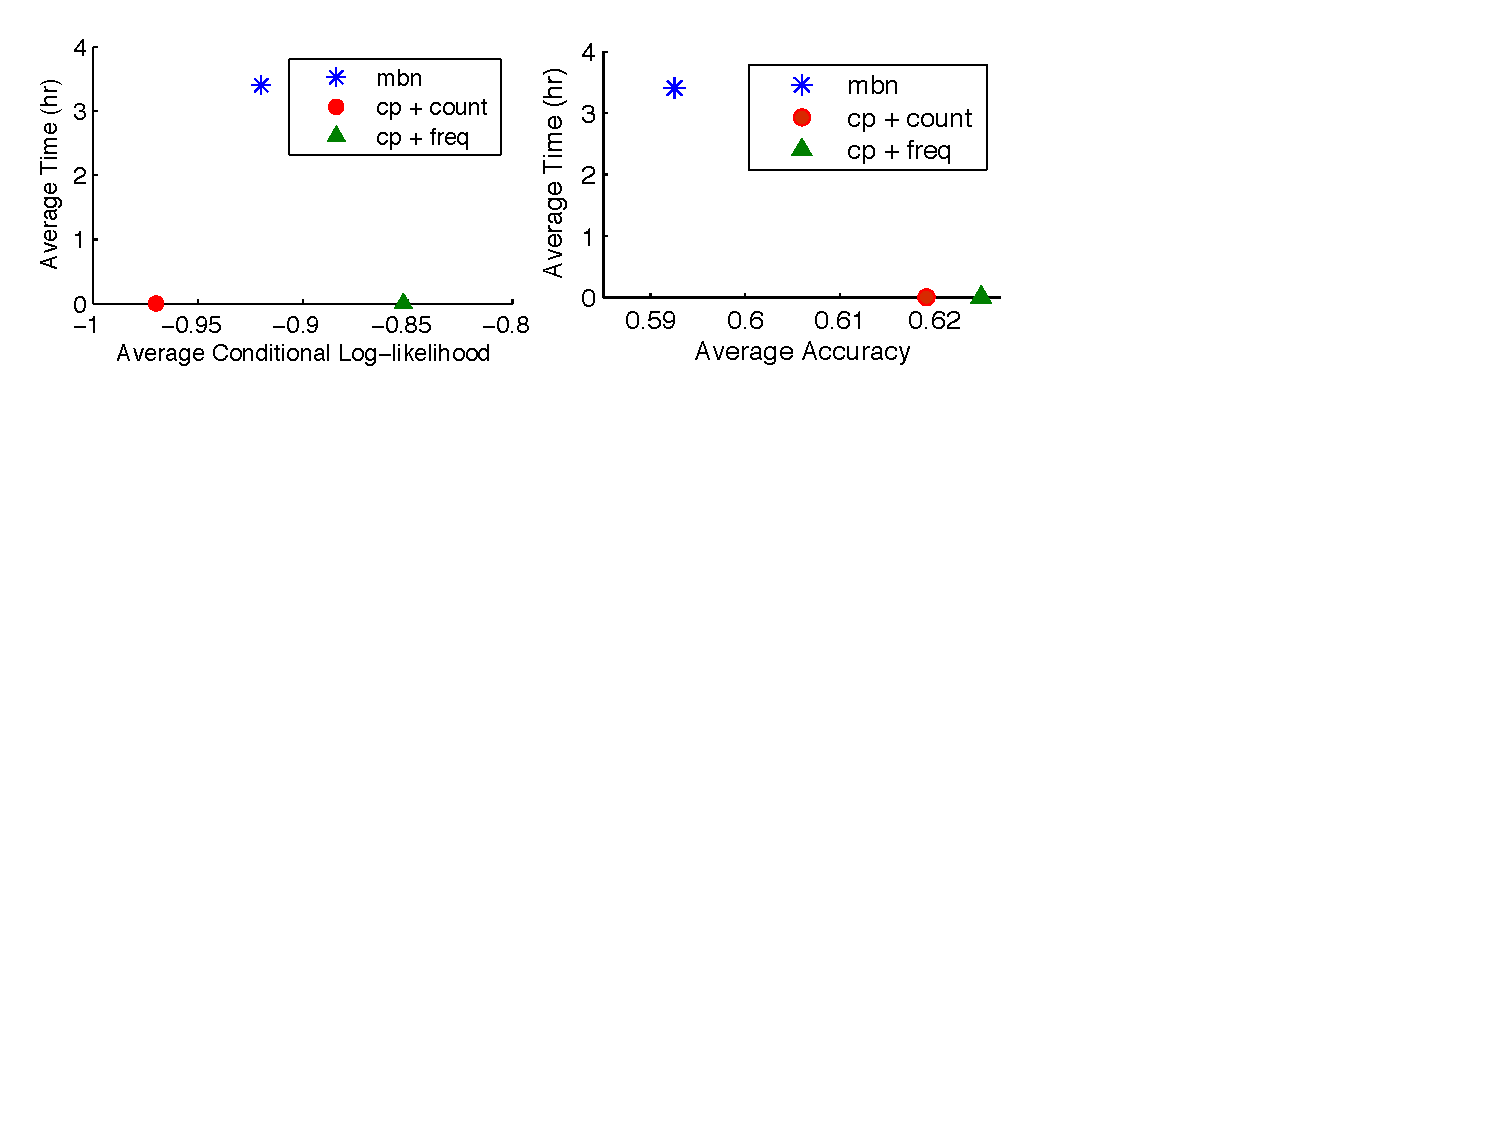
\includegraphics[width=0.5\textwidth]{summary-avg}
%%}
%\caption{Overall predictive performance against weight learning time, averaged over all benchmark databases. 
%%Compared to the Markov Logic methods, Bayes net parameter learning takes essentially no time. 
%\label{fig:summarize}}
%\end{center}
%\end{figure}

\textbf{\em Bayes Net Parameter Learning.} {\em Frequency regression outperforms count regression on every dataset, on both metrics.} The CLL score improves substantially on MovieLens and Hepatitis (by 0.4 resp. 0.13 log-likelihood units). Whereas accuracy is a 0-1 loss function, CLL is continuous, so we expect the balancing of factors to have more impact. 
%
%\subparagraph{CLL.} {\em Using frequencies rather than counts improves the conditional log-likelihood score for the log(cp) weights}, substantially on MovieLens and Hepatitis (by 0.4 resp. 0.13 log-likelihood units). Whereas accuracy is a 0-1 loss function, CLL is continuous, so we expect the balancing of factors to have more impact. 
%%The log-diff method too improves over the log(cp)+count model on all data sets, though not as much as frequency scaling. 
%%These findings support the importance of balancing predictor scales. \marginpar{say something about weights}
%%, either through rescaling (frequency) or adjusting weights (log-diff). 
%
%\subparagraph{Accuracy.}  Frequency regression again outperforms count regression on every dataset.
%, with the exception of Mondial, where the results are essentially the same.
%The Bayes net models have quite similar performance; the general ranking trend  [log(cp) + freq] $>$ [log-diff+ count] $>$ [log(cp) + count] holds for this metric as well, with two exceptions: (1) On Hepatitis, the log-diff model has a slightly higher score than the frequency model (about 0.2\%), and (2) on Movielens, the frequency model has a relatively large 3\% advantage. MovieLens is an especially unbalanced set because the number of ratings varies from movie to movie and user to user.  %\marginpar{More details?} 
%Also, there are generally many more users rating a given movie than movies rated by a given user. 
%The MBN weights in Figure~\ref{fig:boxplots} also indicate that scale balancing is especially important for MovieLens.

\textbf{\em Bayes net vs. Markov net parameters.} 
{\em Bayes net parameters in combination with the frequency/random regression model are competitive with the optimized general weights.} 
 
\subparagraph{CLL.}
The CP+frequency  model scores better than the Markov net weights on Mutagenesis, Hepatitis and MovieLens (by 0.18, 0.11, 0.08 log-likelihood units) but worse on Mondial (0.06 difference). 

%\begin{figure}[htbp]
%\begin{center}
%\resizebox{0.5\textwidth}{!}{
%\includegraphics{summary-cll}
%%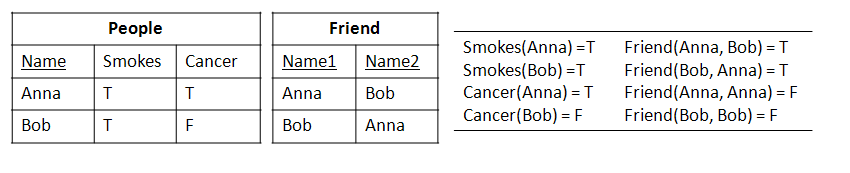
\includegraphics[width=1\textwidth]{database.png}
%}
%\caption{Performance on conditional log-likelihood against time, averaged over all four benchmark databases. \label{fig:summary-cll}}
%\end{center}
%\end{figure}

\subparagraph{Accuracy.} 
The CP+frequency model scores slightly higher than the Markov net weights on every dataset, with the biggest differences on MovieLens (5\%) and Hepatitis (4\%). 

{\em Conclusion.}
The findings support the main claim of our paper, that balancing predictor scales is important for using Bayes net parameters as factors in a log-linear model. Compared to optimized general weights, the BN log-linear model performs very well, which supports its usefulness as a baseline relational model. 


We also performed experiments using the Markov net weights together with the frequency model.
There is little difference between using these weights with counts and frequencies. We hypothesized that the optimized weights already include a scaling component, which explains the equivalence.
This hypothesis is 
%Figure~\ref{fig:boxplots} examines 
confirmed by inspecting the weight magnitudes directly: formulas with many groundings tend to be assigned weights of smaller absolute size. We omit the details due to space constraints. The finding that weights optimized for prediction include a scaling component is further support for the importance of balancing the scales of predictors.



%The scaling effects are especially strong for MovieLens, where the Bayes net frequency model outperforms the count model the most.
%
%Every dataset shows scaling effects except for UW, where all methods achieve the same CLL score. The scaling effects are especially strong for MovieLens, where the Bayes net frequency model outperforms the count model the most.
%
%
%\begin{figure}[htbp]
%\begin{center}
%%\resizebox{0.5\textwidth}{!}{
%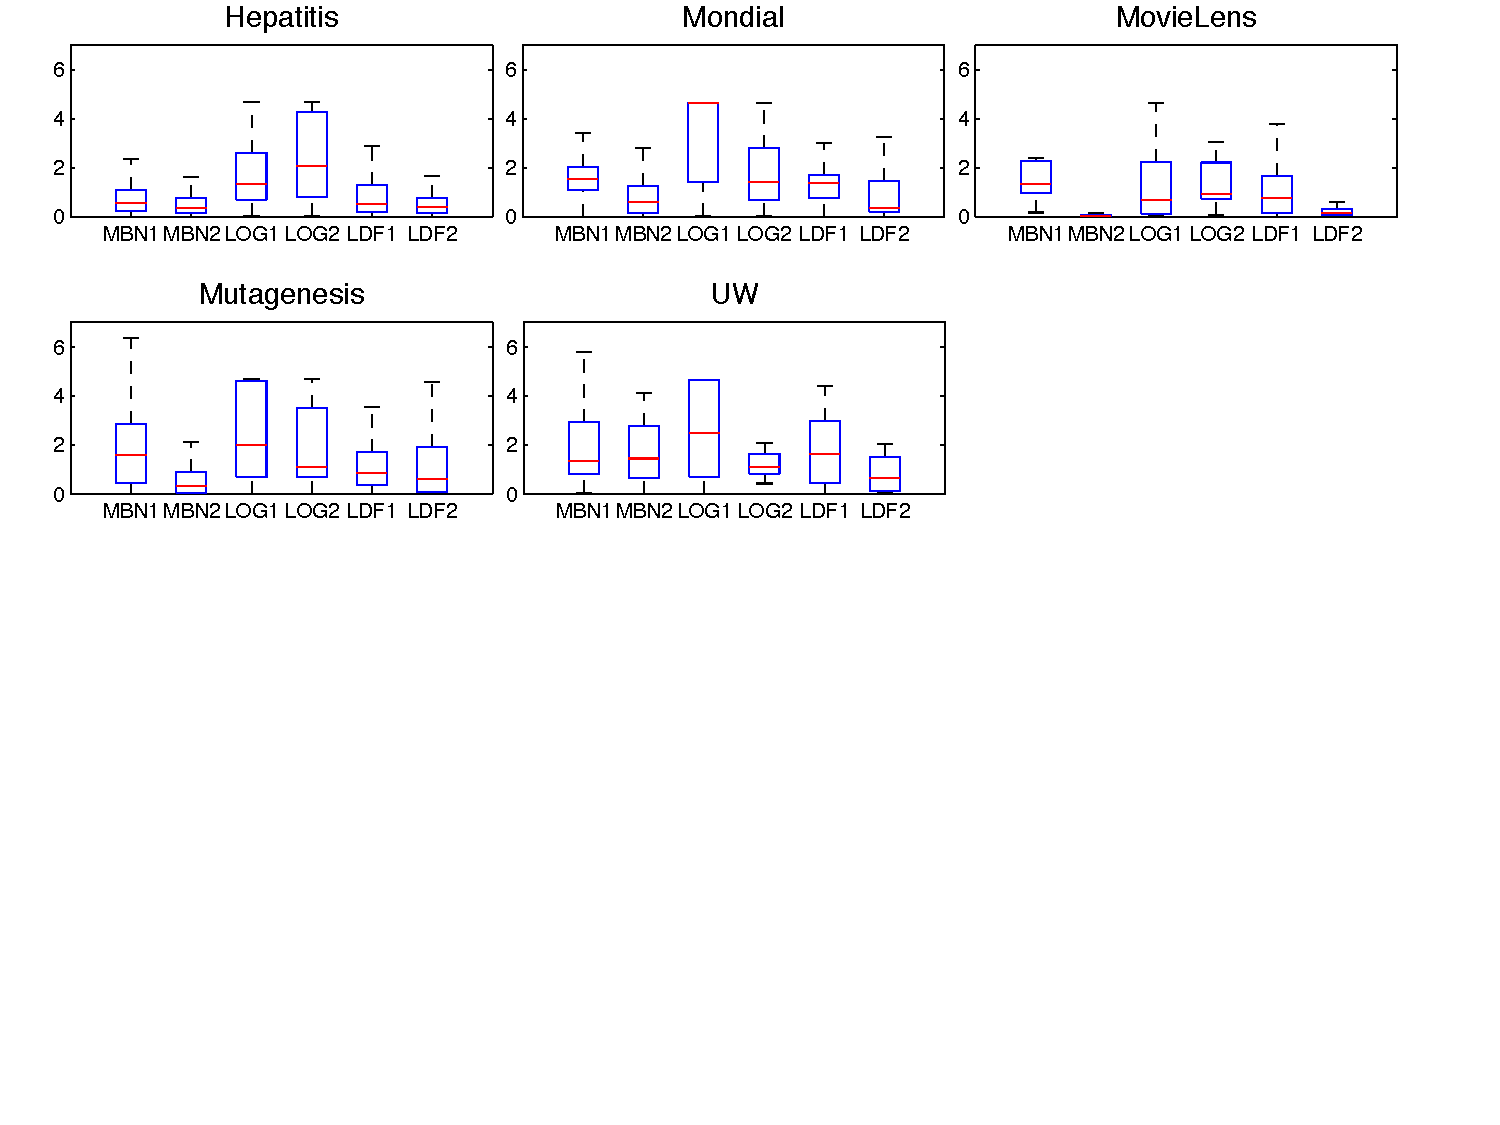
\includegraphics[width=1\textwidth]{boxplots}
%%}
%\caption{Boxplots of the absolute weight sizes learned by the Markov Logic Network method. The median weight size is shown for the set of clauses with one 1st-order variable (left), and the set of clauses with two 1st-order variables (right). Smaller weights for 2-variable clauses balance their larger number of groundings against the smaller number for one-variable clauses.
%\label{fig:boxplots}}
%\end{center}
%\end{figure}


%For the Markov net methods, both count and frequency models have almost the same scores, which is evidence that the learned parameters include scaling components. 
%Overall our experiments provide good evidence that the frequency model using Bayes net conditional probabilities is competitive with a general Markov net log-linear model.


%The next section presents synthetic-data experiments that focus on the scaling effect. 

%\subsubsection{Learning Times.}
%hline Database & Parameters & Complement & FMT & C/FMT \\  \hline \hline
%Mondial & 1618 &157 & 7 &22 \\\hline 
%Hepatitis & 1987 & 18,246 & 77 & 237 \\\hline
%Financial & 10926 & 228,114 & 14,821 &15 \\\hline 
%MovieLens & 326 & 2,070 & 50 & 41 \\ \hline




%\paragraph{Experimental Conclusions.} Compared to Markov Logic parameter learning, Bayes net parameter learning is very fast. The Bayes net parameters were competive with the Markov Logic parameters in terms of predictive performance. Using Bayes net parameters with random/frequency regression outperformed the Markov parameters on all but one dataset on our main metric (CLL). Comparing Bayes net parameters using the frequency vs. count regression, the frequency model has better performance on all datasets on CLL. 
%Together with our analysis of the scale balancing problem,
%the empirical findings make a good case for recommending the frequency model over the count model when the Bayes net parameters are used to derive log-linear weights.



%\begin{figure}[htbp]
%\begin{center}
%\resizebox{0.5\textwidth}{!}{
%\includegraphics{results-summary}
%%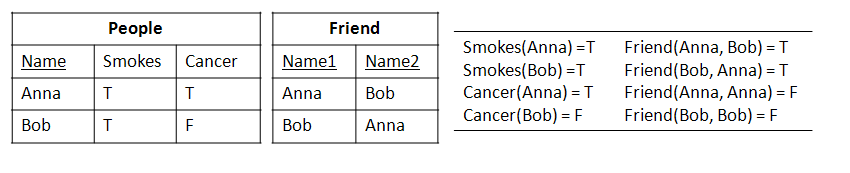
\includegraphics[width=1\textwidth]{database.png}
%}
%\caption{A quick summary of our experimental findings in terms of the average performance over all four benchmark databases. $x$-axis numbers further away from the origin indicate better performance. 
%%The Bayes net parameter methods take next to no time compared to optimizing parameters using Markov Logic procedures. Their predictive performance is better on average than that of the optimized parameters, with the frequency model outperforming the count model.
%\label{fig:summarize}}
%\end{center}
%\end{figure}


%One of the reasons for the widespread popularity of Bayes nets for nonrelational data is that parameters have a natural interpretation and high-quality estimates can be obtained quickly. 
%We believe that providing users with a relational model class that has similar advantages will encourage applications of statistical-relational learning. Users have the option to carry out an initial data exploration and deploy more complex methods if the results are promising.


%\subsection{Synthetic Dataset}
%Scaling factors not so unbalanced. Averages over several predicates. Also has to do with attributes included in Markov blanket. Conduct experiment with synthetic data for the running example.

\section{MLN-Boost Experiments} \label{sec:mln-boost}
MLN-Boost is a state-of-the-art learner for undirected relational models \cite{Khot2011}. To our knowledge, MLN-Boost has not previously been tested on datasets with many descriptive attributes. MLN-Boost simultaneously learns the model structure and parameters,  using functional gradient boosting. 
% to learn models with high predictive accuracy. 
The models are based on ensembles of regression trees rather than Bayes nets, so the model structures are not comparable. Nonetheless, MLN-Boost sets a benchmark for predictive accuracy. We used the Boostr implementation by the inventors of MLN-Boost \cite{Khot2013}. The current version of MLN-Boost is restricted to binary predicates as input. We followed the method of \cite{Khot2011} and converted attributes with $k$ possible values to $k$ binary predicates (value 1 vs. not 1, value 2 vs. not 2,...). 
%This is analogous to converting a $k$-class problem to a set of $k$ one-versus-the-rest binary class problems \cite[Ch.7.1.3]{Bishop}. 
For the predictive accuracy of an attribute with $k$ values, 
%we report two scores: The \textbf{binary} score, which treats each value as defining a one-versus-the-rest binary classification problem, and the \textbf{multi-class} score, where 
we set the acceptance threshold to $1/k$ and check if the model accepts the true attribute value.\footnote{We experimented with different standard methods for extending binary decisions to $k$ classes \cite[Ch.7.1.3]{Bishop2006}, and found that this method gives the best results for MLN-Boost.} We used the inference routine of Boostr. Since inference over the complete dataset is slow, experiments with Boostr challenged our system resources; we tried various settings and report those that yielded the most meaningful results within reasonable computation time ($< 3$ days for a single setting). Including all attributes in the dataset led to an execution error, so we used, for each dataset, two subsets: (1) a {\em maximal} multi-class attribute set with no execution error, and (2) a subset comprising all {\em binary predicates} (e.g., gender). Instead of cross-validation, we use a single random 80-20 training-test split.\footnote{Except for UW where cross-validation is feasible for the maximal set, so we did not use a binary subset.} Boostr was applied to learn a joint model for the selected attributes as targets, with clause-based MLN setting, and default values for options, except for regression trees, where we used as many as possible while obtaining results. 
%(For the binary predicate task 20 trees, for the multi-class task: 10 for UW and Mondial, 5 for Mutagenesis and Hepatitis). 
 Boostr did not terminate on the large dataset MovieLens.

Table~\ref{table:boost-acc} shows the results.  MLN-Boost is much more scalable than previous MLN learning methods, %\cite{Khot2011,Schulte2012}, but 
but still slower than Bayes net learning, by a factor of 10-1,000 depending on the learning task. The number of regression trees has a big impact on learning time. Predictive accuracy for binary attributes (dataset-2) is higher than for multi-class attributes (dataset-2+). The CLL score for BN learning is much better on 2 out of 3 multi-class tasks, and worse on 2 out of 3 binary-class tasks. The scores are comparable only to a limited degree because the BN scores were derived from a joint model of all predicates with cross-validation. Nonetheless, we conclude that our frequency model is very competitive with MLN-Boost, especially for nonbinary attributes.
%The frequency scores are much better the multi-class scores for MLN-Boost. The frequency scores are competitive for the binary class scores of MLN-Boost, which is a good result since the frequency model provides true multi-class predictions. 
%Future work on a multi-class extension of MLN-Boost would permit a more direct comparison. 
A multi-class extension of MLN-Boost would permit a more direct comparison; we leave this for future work.
 
 \begin{table}[htdp]
\caption{Performance Metrics for MLN-Boost. NT = inference did not terminate.}
\begin{center}
\resizebox{0.5\textwidth}{!}{
\begin{tabular}{|c|c|c|c|c|c|}
\hline
Task & 
\begin{tabular}{c}
\#Attributes/ \\
\#Predicates
\end{tabular}
 & \begin{tabular}{c}
Learning/ \\
\#Trees
\end{tabular}
& ACC & CLL & \begin{tabular}{c}
Bayes Net: \\
$\log$(cp)+freq
\end{tabular} \\\hline
UW-2+ & 4/11 & 1018.25 s/10 & 27.68\% & -1.74 & \textbf{-0.41} \\\hline
Mondial-2+ & 7/31 & 314 s/10 & 34.77\% & -2.72 & \textbf{-1.36} \\\hline
Mondial-2 & 1 & 260.2 s/20 & 80.77\% & \textbf{-0.24} & -1.36 \\\hline
Muta-2+ & 3/7 & 1589 s/5 & 46.19\% & \textbf{-0.63} & -0.73 \\\hline
Muta-2 & 4 & 94389.2 s/20 & 68.98\% & \textbf{-0.53} & -0.73 \\\hline
Hepatitis-2+ & 13/37  & 9791s/5 & NT & NT & -1.07 \\\hline
Hepatitis-2 & 5 & 19921 s/20 & 30.08\% & -1.53 & \textbf{-1.07} \\\hline
\end{tabular}
}
\end{center}
\label{table:boost-acc}
\end{table}%

 
 
 

 
 
%Another promising direction is to combine our frequency model with the powerful technique of functional gradient boosting. Frequencies can be used instead of counts to define the gradient; conversely, gradient boosting could learn ensembles of Bayes net models.
%
%\begin{table}[t]
%\caption{Predictive accuracy of MLN-Boost}
%\begin{center}
%\begin{large}
%\resizebox{0.5\textwidth}{!}{
%\begin{tabular}{|c|c|c|c|c|c|}
%CLL & UW & Mondial & MovieLens & Mutagenesis & Hepatitis \\\hline
%Binary & -0.44 $\pm$ 0.07 & \textbf{-1.25} $\pm$ 0.04 & -0.79 $\pm$ 0.03 & -0.91 $\pm$ 0.09 & -1.18 $\pm$ 0.26 \\ \hline
%%mbn+freq & -0.43 $\pm$ 0.07 & \textbf{-1.28} $\pm$ 0.07 & -0.83 $\pm$ 0.03 & -0.93 $\pm$ 0.13 & -1.16 $\pm$ 0.21 \\
%%%mbn+freq & -0.43 $\pm$ 0.07 & \textbf{-1.28} $\pm$ 0.07 & -0.83 $\pm$ 0.03 & -0.93 $\pm$ 0.13 & -1.16 $\pm$ 0.21 \\
%Multi & -0.47 $\pm$ 0.10 & -1.39 $\pm$ 0.19 & -1.19 $\pm$ 0.07 & -0.84 $\pm$ 0.03 & -1.33 $\pm$ 0.07 \\
%%log-diff+cnt & -0.42 $\pm$ 0.05 & -1.36 $\pm$ 0.11 & -1.10 $\pm$ 0.16 & -0.77 $\pm$ 0.03 & -1.20 $\pm$ 0.07 \\
%%%log(cp)+freq & \textbf{-0.41} $\pm$ 0.04 & -1.34 $\pm$ 0.09 & \textbf{-0.71} $\pm$ 0.01 & \textbf{-0.73} $\pm$ 0.04 & \textbf{-1.07} $\pm$ 0.10 \\\hline
%\hline
%\end{tabular}}
%\end{large}
%\end{center}
%\label{table:boost-acc}
%\begin{center}
%\begin{large}
%
%\resizebox{0.5\textwidth}{!}{
%\begin{tabular}{|c|c|c|c|c|c|}
%Accuracy& UW & Mondial & MovieLens & Mutagenesis & Hepatitis \\\hline
%Binary & 80.3\% $\pm$ 0.05 & 47.8\% $\pm$ 0.03 & 59.7\% $\pm$ 0.02 & 61.5\% $\pm$ 0.02 & 51.0\% $\pm$ 0.02 \\\hline
%%mbn+freq & 80.25\% $\pm$ 0.05 & 43.81\% $\pm$ 0.04 & 58.76\% $\pm$ 0.02 & 60.89\% $\pm$ 0.03 & 50.94\% $\pm$ 0.02 \\
%Multi & 78.3\% $\pm$ 0.08 & 48.4\% $\pm$ 0.02 & 64.3\% $\pm$ 0.01 & 61.4\% $\pm$ 0.05 & 49.2\% $\pm$ 0.03 \\
%%%log(cp)+cnt & 78.3\% $\pm$ 0.08 & \textbf{44.7\%} $\pm$ 0.04 & 64.3\% $\pm$ 0.01 & 61.4\% $\pm$ 0.05 & 49.2\% $\pm$ 0.03 \\
%%log-diff+cnt & 80.9\% $\pm$ 0.06 & \textbf{44.7\%} $\pm$ 0.04 & 61.9\% $\pm$ 0.02 & \textbf{67.0\%} $\pm$ 0.03 & \textbf{55.1\%} $\pm$ 0.02 \\
%%%log(cp)+freq & \textbf{81.0\%} $\pm$ 0.06 & 44.6\% $\pm$ 0.04 & \textbf{65.1\%} $\pm$ 0.01 & \textbf{67.0\%} $\pm$ 0.03 & \textbf{54.8\%} $\pm$ 0.02 \\
%\hline
%\end{tabular}
%}
%\end{large}
%\end{center}
%\end{table}%

\section{Conclusion and Future Work} %Inference and Consistency.
This paper presented a new log-linear inference model for Bayes nets applied to relational data. In a Bayes net model, the weight parameters are log-conditional probabilities of parents given children. An innovation of our model is to  use  the frequencies of relational patterns as predictor variables, rather than their counts as in previous log-linear models.
%The predictor variables in previous relational log-linear models are instance counts of relational patterns. 
%We provided theoretical considerations and empirical evidence that for conditional probability parameters, it is important to rescale the predictors to be instance frequencies. 
Using frequencies rather than counts addresses the imbalance problem, that counts of different features may be on very different scales. In empirical tests of predictive performance, frequencies outperformed counts on all datasets. 
A novel sampling semantics for the frequency model shows that it can be interpreted as the expected value of applying Bayes net prediction to a random instantiation of a target node's Markov blanket. Thus while the change from counts to frequencies is a small alteration in the form of the predictive equations, it leads to a different semantics, and it has a big impact on predictive performance.
Using the maximum likelihood values as Bayes net parameters is much faster than optimizing weights using standard Markov Logic methods, typically seconds vs. hours. 

A topic for future work is to investigate the extension of the local probability models to joint inferences. Local probability models may be inconsistent in the sense that there is no joint distribution that agrees with the local conditional probabilities \cite{Heckerman2000}. An open theoretical question is whether frequency regression models for different target nodes are guaranteed to be mutually consistent. If they are inconsistent, a possible approach is to apply the recent averaging methods for dependency networks \cite{Lowd2012}.

% The key idea is to consider the expected log-linear regression value from a {\em random} instantiation of a node's Markov blanket. We provided an equivalent closed form definition that is a log-linear model, whose predictor variables are scaled to be frequencies in the range [0,1]. We compared random regression with standard log-linear models, using as weights both empirical conditional probabilities and weights learned by local optimization. 
%The log-conditional probabilities are much faster to compute, typically seconds vs. hours. The predictive performance of log-conditional probability weights was competitive with optimized regression weights, in fact superior on all but one dataset. Overall, random regression appears to be a principled, fast, and accurate model for relational prediction with Bayes nets.
%
%PBNs have been extended with decision trees to obtain more compact models of the conditional distribution of a child node given its parents \cite{Khosravi2012}. This is a natural extension for testing the random regression model; we hypothesize that scaling is even more important, because decision tree pruning leads to more variation in clause length. The powerful and effective technique of functional gradient boosting \cite{Khot2011} could be applied to learning tree models that augment a Bayes net; gradient boosting is well-suited to learning potential functions for log-linear models. 
%In sum, random regression offers a tractable and intuitive definition of inference for Bayes nets that is well-defined even in the presence of cyclic dependencies. 


%% The file named.bst is a bibliography style file for BibTeX 0.99c
\bibliographystyle{named}
\bibliography{master}
\end{document}

